\documentclass[11pt]{article}

\textheight=23cm \textwidth=16cm
\topmargin=-1cm
\oddsidemargin=0pt \evensidemargin=0pt \marginparwidth=2cm

\usepackage{epsfig}

\newcommand{\func}[1]{\texttt{#1}}
\newcommand{\ie}{\hbox{\textit{i.e.}}\ }
\newcommand{\eg}{\hbox{\textit{e.g.}}\ }

\title{Metanet User's Guide and Tutorial}
\author{Claude Gomez \and Maurice Goursat}
\date{Manual version 1.1 for Scilab 2.4}

\makeindex

\begin{document}

\maketitle

Metanet is a toolbox of Scilab for graphs and networks computations.
It comes as new
Scilab functions together with a graphical
window for displaying and modifying graphs.

You can use the Metanet toolbox in Scilab without using the graphical window
window at all,
\ie without seeing the graphs or the networks you are working with.

\section{Representation of graphs}

The graphs handled by Metanet are directed or undirected multigraphs 
(loops are allowed).
A \emph{graph}\index{graph}
is a set of arcs and nodes. 

A graph must have at least one arc. 
We call \emph{arc}\index{arc} a directed link between two nodes. 
For instance the arc $(i,j)$ goes from \emph{tail}\index{node!tail}
node $i$ to \emph{head}\index{node!head}
node $j$. 
We call \emph{edge}\index{edge} the 
corresponding undirected link. A minimal way to represent a graph is to
give the number of nodes, the list of the tail nodes and the list of the
head nodes. Each node has a number and each arc has a number. The numbers
of nodes are consecutive and the number of arcs are consecutive. In Scilab,
these lists are represented by row vectors. So, if we call \texttt{tail} and
\texttt{head} these row vectors, the arc number $i$ goes from node
number \texttt{tail(i)} to node number \texttt{head(i)}. Moreover, 
it is necessary to give the number of
nodes, because isolated nodes\index{node!isolated}  
(without any arc) can exist. The
size of the vectors \texttt{tail} and \texttt{head} is the number of
edges of the graph. This is the standard representation of graphs in
Metanet as it is described in the graph list (see \ref{graph-list}).
There are functions to compute other representations better suited for
some algorithms (see \ref{representation}).

The distinction between edges\index{edge} and arcs is meaningful when
we 
deal with
undirected graphs. This distinction is not needed when we
only use the standard functions of Metanet. There is no distinction
between an \emph{arc}\index{arc} and a \emph{directed edge}\index{directed
edge}. 
We will often use indistinctly
these two terms.

A new object, the graph list data structure, is defined in
Scilab to handle graph. It is described below.

\subsection{The graph list data structure} \label{graph-list}
Metanet uses the graph list data structure to represent graphs.
With this type of description (see~\ref{representation}), we can 
have directed or undirected
multigraphs and multiple loops are allowed.
The graph list data structure is a typed list. 
As usual, the first element of this object is itself a list which
defines its 
type, \texttt{'graph'}, 
and all the access functions to the other elements.
The graph list has 33 elements (not counting the first one defining the type).
Only the first five elements must have a value in the list,
all the others can be given the empty vector \texttt{[]} as a value, and then a
default is used. These five required elements are:
\begin{description}
  \item[name] name of the graph (a string)
  \item[directed] flag equal to 1 if the graph is directed or equal
  to 0 if the graph is undirected
  \item[node\_number] number of nodes
  \item[tail] row vector of the tail node numbers
  \item[head] row vector of the head node numbers
\end{description}
\noindent A graph must at least have one arc, so \texttt{tail} and 
\texttt{head}
cannot be empty. 


For instance, you can define a graph list (see \ref{creating}) by
\begin{verbatim}
g=make_graph('min',1,1,[1],[1]);
\end{verbatim}
which is the simplest graph you can create (it is directed, has 
one node and one loop arc on this node).

Each element of the list can be accessed by using its name.
For instance, if \texttt{g} is a graph list and
you want to get the \texttt{node\_number} element, you only have to type:\\
\texttt{g('node\_number')}\\
and if you want to change this value to 10, you only have to type:\\
\texttt{g('node\_number')=10}

The \func{check\_graph} function checks a graph list to see if
there are inconsistencies in its elements. Checking is not only
syntactic (number of elements of the list, compatible sizes 
of the vectors), but also semantic in the sense that 
\func{check\_graph} checks that \texttt{node\_number}, \texttt{tail} and 
\texttt{head} elements of the list can really represent a  graph.
This checking is automatically made when calling functions with a
graph list as an argument.

You will find below the description of all the elements of a graph list.
Each element is described by one or more lines.
The first lines give the name of the element and
its definition, with its Scilab type if
needed.
The last line gives the default for elements that can have one.
The name of the element is used to access 
the elements
of the list.

\begin{description}
  \item[name] 

Name of the graph; a string with a maximum of 80
characters (\emph{REQUIRED}).

  \item[directed]

Flag giving the type of the graph; it is equal to 1 if the graph is
directed or equal to 0 is the graph is undirected (\emph{REQUIRED}).

  \item[node\_number]

Number of nodes (\emph{REQUIRED}).

  \item[tail]

Row vector of the tail node numbers (\emph{REQUIRED}).

  \item[head]

Row vector of the head node numbers (\emph{REQUIRED}).

  \item[node\_name]

Row vector of the node names; they \emph{MUST} be different.

Default is the node numbers as node names.

  \item[node\_type]

Row vector of the node types; the type is an integer from 0 to 2:
\begin{itemize}
  \item[0:] plain node
  \item[1:] sink node
  \item[2:] source node
\end{itemize}

This element is mainly used to draw the nodes in the Metanet
window. A plain node is drawn as a circle. A sink or source node is a
node where extraneous flow goes out the node or goes into the node; it
is drawn differently (a circle with an outgoing or ingoing arrow).

Default is 0 (plain node).

  \item[node\_x]

Row vector of the x coordinates of the nodes.

Default is computed when showing the graph in the Metanet window
(see \ref{xmetanet}).

  \item[node\_y]

Row vector of the y coordinates of the nodes.

Default is computed when showing the graph in the Metanet window
(see \ref{xmetanet}).

  \item[node\_color]

Row vector of the node colors; 
the color is an integer from 0 to 16:
\begin{itemize}
  \item[0:] black
  \item[1:] navyblue
  \item[2:] blue
  \item[3:] skyblue
  \item[4:] aquamarine
  \item[5:] forestgreen
  \item[6:] green
  \item[7:] lightcyan
  \item[8:] cyan
  \item[9:] orange
  \item[10:] red
  \item[11:] magenta
  \item[12:] violet
  \item[13:] yellow
  \item[14:] gold
  \item[15:] beige
  \item[16:] white
\end{itemize}

Default is 0 (black).

  \item[node\_diam]

Row vector of the sizes of the node diameters in pixels (a node is
drawn as a circle).

Default is the value of element \texttt{default\_node\_diam}.

  \item[node\_border]

Row vector of the sizes of the node borders in pixels.

Default is the value of element \texttt{default\_node\_border}.

  \item[node\_font\_size]

Row vector of the sizes of the font used to draw the name or the label
of the node; 
you can choose
8, 10, 12, 14, 18 or 24.

Default is the value of element \texttt{default\_font\_size}.

  \item[node\_demand]

Row vector of the node demands.

The demands of the nodes are used in functions
\func{min\_lcost\_cflow}, 
\func{min\_lcost\_flow1}, \func{min\_lcost\_flow2},
\func{min\_qcost\_flow} and
\func{supernode}.

Default is 0.

  \item[edge\_name]

Row vector of the edge names; edge names need not be different.

Default is the edge numbers as edge names.

  \item[edge\_color]

Row vector of the edge colors; 
the color is an integer from 0 to 16 (see \texttt{node\_color}).

Default is 0 (black).

  \item[edge\_width]

Row vector of the sizes of the edge widths in pixels.

Default is the value of element \texttt{default\_edge\_width}.

  \item[edge\_hi\_width]

Row vector of the sizes of the highlighted edge widths in pixels.

Default is the value of element \texttt{default\_edge\_hi\_width}.

  \item[edge\_font\_size]

Row vector of the sizes of the font used to draw the name or the label of
the edge; you 
can choose 8, 10, 12, 14, 18 or 24.

Default is the value of element \texttt{default\_font\_size}.

  \item[edge\_length]

Row vector of the edge lengths.

The lengths of the edges are used in functions \func{graph\_center}, 
\func{graph\_diameter},
\func{salesman} and \func{shortest\_path}.

Default is 0.

  \item[edge\_cost]

Row vector of the edge costs.

The costs of the edges are used in functions \func{min\_lcost\_cflow}, 
\func{min\_lcost\_flow1} and \func{min\_lcost\_flow2}.

Default is 0.

  \item[edge\_min\_cap]

Row vector of the edge minimum capacities.

The minimum capacities of the edges are used in functions \func{max\_flow}, 
\func{min\_lcost\_cflow}, 
\func{min\_lcost\_flow1}, \func{min\_lcost\_flow2} and
\func{min\_qcost\_flow}.

Default is 0.

  \item[edge\_max\_cap]

Row vector of the edge maximum capacities.

The maximum capacities of the edges are used in functions 
\func{max\_cap\_path}, 
\func{max\_flow}, 
\func{min\_lcost\_cflow}, 
\func{min\_lcost\_flow1}, \func{min\_lcost\_flow2} and
\func{min\_qcost\_flow}.

Default is 0.

  \item[edge\_q\_weight]

Row vector of the edge quadratic weights. It corresponds to $w(u)$ in
the value of the cost on edge $u$ with flow $\varphi(u)$:
$\frac{1}{2}w(u)(\varphi(u)-w_0(u))^2$.

The quadratic weights of the edges are used in function 
\func{min\_qcost\_flow}.

Default is 0.

  \item[edge\_q\_orig]

Row vector of the edge quadratic origins. It corresponds to $w_0(u)$ in
the value of the cost on edge $u$ with flow $\varphi(u)$:
$\frac{1}{2}w(u)(\varphi(u)-w_0(u))^2$.

The quadratic origins of the edges are used in function 
\func{min\_qcost\_flow}.

Default is 0.

  \item[edge\_weight]

Row vector of the edge weights.

The weights of the edges are used in function
\func{min\_weight\_tree}.

Default is 0.

  \item[default\_node\_diam]

Default size in pixels of the node diameters of the graph.

Default is 20.

  \item[default\_node\_border]

Default size in pixels of the node borders of the graph.

Default is 2.

  \item[default\_edge\_width]

Default size in pixels of the edge widths of the graph.

Default is 1.

  \item[default\_edge\_hi\_width]

Default size in pixels of the highlighted edge widths of the graph.

Default is 3.

  \item[default\_font\_size]

Default size of the font used to draw the names or the labels of nodes
and edges.

Default is 12.

  \item[node\_label]

Row vector of the node labels.

Node labels are used to draw a string in a node. It can be any string.
An empty label can be given as a blank string \texttt{' '}.

  \item[edge\_label]

Row vector of the edge labels.

Edge labels are used to draw a string on an edge. It can be any string.
An empty label can be given as a blank string \texttt{' '}.

\end{description}

\subsection{Various representations of graphs}\label{representation}

\subsubsection{Names and numbers}\label{number}

First of all, we need to distinguish between the name of a node or the
name of an
edge and their internal numbers\index{internal number}. 
The name can be any string. Its is saved
in the graph file (see~\ref{loading}).
The internal
number is generated automatically when loading a graph. The nodes and
the edges have 
consecutive internal numbers starting from 1. 
When using the Scilab functions working on graphs, \emph{all the
computations are made with internal numbers}.

It is very important to give different names to the nodes because the
nodes are distinguished by their names when they are loaded. This
distinction is not important for edges.

Often, the names are taken as the internal numbers. This is
the default when no names are given. In this case, the distinction
between a name and a number is not meaningful. Only the type of the
variable is not the same: the name is a string and the number is an integer.

In the following when
we talk about the number of a node or the number of an edge, we mean
the internal number.

\subsubsection{Tail head}

We have seen that the standard representation of a graph used by
Metanet is by the means of two row vectors
\texttt{tail} and
\texttt{head}:
arc number $i$ goes from node
number \texttt{tail(i)} to node number \texttt{head(i)}.
The size of these vectors is the same and is the number of arcs of the
graph.

Moreover the number of nodes must be given. It is greater than or
equal to the maximum integer number in \texttt{tail} and
\texttt{head}. If node numbers do not belong to \texttt{tail} and
\texttt{head} then there are isolated nodes.

If the graph is undirected, it is the same, but \texttt{tail(i)} and
\texttt{head(i)} can be exchanged.

This representation is very general and gives directed or undirected
multigraphs with possible loops and isolated nodes.

The standard function to create graphs is \func{make\_graph}
(see~\ref{creating}). 
For instance, we can create a small directed graph with a loop and an
isolated  node (see figure~\ref{fig-foo}) by using:\\
node number = 4, tail = [1,1,2,3], head = [2,3,1,3],\\
or in Scilab:\\
\texttt{g=make\_graph('foo',1,4,[1 1 2 3],[2 3 1 3]);}

\begin{figure}
 \begin{center}\input{foo.pstex_t}\end{center}
 \caption{Small directed graph}
 \label{fig-foo}
\end{figure}

\subsubsection{Adjacency lists}\label{adjacency}

Another interesting representation often used by algorithms is the
\emph{adjacency lists}\index{adjacency lists} representation. 
It uses three row vectors, \texttt{lp},
\texttt{ls} and \texttt{la}. If $n$ is the number of nodes and $m$ is the number
of arcs of the graph:\\
\texttt{lp} is the pointer  array  (size = $n+1$)\\
\texttt{ls} is the node array (size = $m$)\\
\texttt{la} is the arc array (size = $m$).\\
If the graph is undirected, each edge corresponds to two arcs.

With this type of representation, it is easy to know the successors of
a node. Node number \texttt{i} has \texttt{lp(i+1)-lp(i)} successors
nodes with numbers from
\texttt{ls(lp(i))} to \texttt{ls(lp(i+1)-1)},
the corresponding arcs are have numbers from 
\texttt{la(lp(i))} to \texttt{la(lp(i+1)-1)}.

The adjacency lists representation of the graph of figure~\ref{fig-foo}
is given below:

\begin{center}
\setlength{\unitlength}{0.00083300in}%
%
\begingroup\makeatletter\ifx\SetFigFont\undefined%
\gdef\SetFigFont#1#2#3#4#5{%
  \reset@font\fontsize{#1}{#2pt}%
  \fontfamily{#3}\fontseries{#4}\fontshape{#5}%
  \selectfont}%
\fi\endgroup%
\begin{picture}(2712,2421)(1201,-2323)
\thicklines
\put(2551,-1411){\framebox(450,450){}}
\put(1651,-2311){\framebox(450,450){}}
\put(1651,-1411){\framebox(450,450){}}
\put(2101,-1411){\framebox(450,450){}}
\put(3001,-1411){\framebox(450,450){}}
\put(2101,-2311){\framebox(450,450){}}
\put(2551,-2311){\framebox(450,450){}}
\put(3001,-2311){\framebox(450,450){}}
\put(2101,-511){\framebox(450,450){}}
\put(1651,-511){\framebox(450,450){}}
\put(2551,-511){\framebox(450,450){}}
\put(3001,-511){\framebox(450,450){}}
\put(3451,-511){\framebox(450,450){}}
\put(1876,-511){\vector( 0,-1){450}}
\put(1876,-1411){\line( 0,-1){450}}
\put(2326,-1411){\line( 0,-1){450}}
\put(2776,-1411){\line( 0,-1){450}}
\put(3226,-1411){\line( 0,-1){450}}
\put(2326,-511){\line( 0,-1){300}}
\put(2326,-811){\line( 1, 0){450}}
\put(2776,-811){\vector( 0,-1){150}}
\put(2776,-511){\line( 0,-1){150}}
\put(2776,-661){\line( 1, 0){450}}
\put(3226,-661){\vector( 0,-1){300}}
\put(1801,-361){\makebox(0,0)[lb]{\smash{\SetFigFont{12}{14.4}{\rmdefault}{\mddefault}{\updefault}1}}}
\put(2251,-361){\makebox(0,0)[lb]{\smash{\SetFigFont{12}{14.4}{\rmdefault}{\mddefault}{\updefault}3}}}
\put(2701,-361){\makebox(0,0)[lb]{\smash{\SetFigFont{12}{14.4}{\rmdefault}{\mddefault}{\updefault}4}}}
\put(3151,-361){\makebox(0,0)[lb]{\smash{\SetFigFont{12}{14.4}{\rmdefault}{\mddefault}{\updefault}5}}}
\put(3601,-361){\makebox(0,0)[lb]{\smash{\SetFigFont{12}{14.4}{\rmdefault}{\mddefault}{\updefault}5}}}
\put(1801,-1261){\makebox(0,0)[lb]{\smash{\SetFigFont{12}{14.4}{\rmdefault}{\mddefault}{\updefault}2}}}
\put(2251,-2161){\makebox(0,0)[lb]{\smash{\SetFigFont{12}{14.4}{\rmdefault}{\mddefault}{\updefault}2}}}
\put(2251,-1261){\makebox(0,0)[lb]{\smash{\SetFigFont{12}{14.4}{\rmdefault}{\mddefault}{\updefault}3}}}
\put(2701,-1261){\makebox(0,0)[lb]{\smash{\SetFigFont{12}{14.4}{\rmdefault}{\mddefault}{\updefault}1}}}
\put(3151,-1261){\makebox(0,0)[lb]{\smash{\SetFigFont{12}{14.4}{\rmdefault}{\mddefault}{\updefault}3}}}
\put(1801,-2161){\makebox(0,0)[lb]{\smash{\SetFigFont{12}{14.4}{\rmdefault}{\mddefault}{\updefault}1}}}
\put(2701,-2161){\makebox(0,0)[lb]{\smash{\SetFigFont{12}{14.4}{\rmdefault}{\mddefault}{\updefault}3}}}
\put(3151,-2161){\makebox(0,0)[lb]{\smash{\SetFigFont{12}{14.4}{\rmdefault}{\mddefault}{\updefault}4}}}
\put(1801, 14){\makebox(0,0)[lb]{\smash{\SetFigFont{10}{12.0}{\rmdefault}{\mddefault}{\updefault}1}}}
\put(2251, 14){\makebox(0,0)[lb]{\smash{\SetFigFont{10}{12.0}{\rmdefault}{\mddefault}{\updefault}2}}}
\put(2701, 14){\makebox(0,0)[lb]{\smash{\SetFigFont{10}{12.0}{\rmdefault}{\mddefault}{\updefault}3}}}
\put(3151, 14){\makebox(0,0)[lb]{\smash{\SetFigFont{10}{12.0}{\rmdefault}{\mddefault}{\updefault}4}}}
\put(3601, 14){\makebox(0,0)[lb]{\smash{\SetFigFont{10}{12.0}{\rmdefault}{\mddefault}{\updefault}5}}}
\put(1201,-286){\makebox(0,0)[lb]{\smash{\SetFigFont{14}{16.8}{\rmdefault}{\mddefault}{\updefault}lp}}}
\put(1201,-1186){\makebox(0,0)[lb]{\smash{\SetFigFont{14}{16.8}{\rmdefault}{\mddefault}{\updefault}ls}}}
\put(1201,-2086){\makebox(0,0)[lb]{\smash{\SetFigFont{14}{16.8}{\rmdefault}{\mddefault}{\updefault}la}}}
\end{picture}

\end{center}

The function used to compute the adjacency list
representation of a graph is \func{adj\_lists}.

\subsubsection{Node-arc matrix}

For a directed graph,
if $n$ is the number of nodes and $m$ is the number of arcs of the
graph, the node-arc matrix\index{node-arc matrix} $A$ is a $n\times m$ 
matrix:\\
if $A(i,j)=+1$, then node $i$ is the tail of arc $j$\\
if $A(i,j)=-1$, then node $i$ is the head of arc $i$.\\
If the graph is undirected and $m$ is the number of edges, 
the node-arc matrix $A$ is also a $n\times m$ matrix and:\\
if $A(i,j)=1$, then node $i$ is an end of edge $j$.

With this type of representation, it is impossible to have loops.

This matrix is represented in Scilab as a sparse matrix.

For instance, the node-arc matrix corresponding to figure~\ref{fig-foo},
with loop arc number 4 deleted is :
\[\left(\begin{array}{rrr}
 1 &  1 & -1 \\
-1 &  0 &  1 \\
 0 & -1 &  0 \\
 0 &  0 &  0 \\
\end{array}\right)\]

If the same graph is undirected, the matrix is:
\[\left(\begin{array}{ccc}
 1 &  1 &  1 \\
 1 &  0 &  1 \\
 0 &  1 &  0 \\
 0 &  0 &  0 \\
\end{array}\right)\]

The functions used to compute the node-arc matrix
of a graph, and to come back to a graph from the node-arc matrix are
\func{graph\_2\_mat} and \func{mat\_2\_graph}.

\subsubsection{Node-node matrix}

The $n\times n$ node-node
matrix\index{node-node matrix} of the
graph is the matrix $A$ where $A(i,j)=1$ if there is one arc from node $i$ to 
node
$j$. Only 1 to 1
graphs (no more than one arc from one node to another) can be
represented, but loops are allowed.
This matrix is also known as the ``adjacency matrix''.

The same functions used to compute the node-arc matrix
(see above) of a graph are used to compute the node-node
matrix: \texttt{graph\_2\_mat}
and \texttt{mat\_2\_graph}. To
specify that we are working with the node-node matrix, the flag
\texttt{'node\-node'} must be given as the last argument of these
functions.

For instance, you can find below the node-node  matrix of the graph
corresponding to Figure~\ref{fig-foo}:
\[\left(\begin{array}{cccc}
 0 & 1 & 1 & 0 \\
 1 & 0 & 0 & 0 \\
 0 & 0 & 1 & 0 \\
 0 & 0 & 0 & 0 \\
\end{array}\right)\]

and the node-node matrix for the same undirected graph:
\[\left(\begin{array}{cccc}
 0 & 1 & 1 & 0 \\
 1 & 0 & 0 & 0 \\
 1 & 0 & 1 & 0 \\
 0 & 0 & 0 & 0 \\
\end{array}\right)\]

\subsubsection{Chained lists}

Another representation used by some algorithms is given by the
\emph{chained lists}\index{chained lists}. 
This representation uses four vectors,
\texttt{fe}, \texttt{che}, \texttt{fn} and \texttt{chn} which are
described below:\\
\texttt{e1=fe(i))} is the number of the first edge starting from node 
\texttt{i}\\
\texttt{e2=che(e1)} is the number of the second edge starting from
node \texttt{i}\\
\texttt{e3=che(e2)} is the number of the third edge starting from
node \texttt{i} \\
and so on until the value is 0\\
\texttt{fn(i)} is the number of the first node reached from node i\\
\texttt{chn(i)} is the number of the node reached by edge
\texttt{che(i)}.

All this can be more clearly seen on figure~\ref{fig-chain}.


\begin{figure}
  \begin{center}\input{chain.pstex_t}\end{center}
  \caption{Chained lists representation of graphs}
  \label{fig-chain}
\end{figure}

You can use the \func{chain\_struct} function to obtain the chained
lists representation of a graph from the adjacency lists representation
(see~\ref{adjacency}).

\section{Managing graphs}

We have seen (see~\ref{graph-list}) that a graph in Scilab is
represented by a graph list. This list contains everything needed to
define the graph, arcs, nodes, coordinates, colors, attributes, width of the
arcs, etc.

To create, load and save graphs in Scilab, you can use only Scilab
functions, handling graph lists, or you can use the Metanet window.
We describe here the first way. For the second way, see~\ref{xmetanet}.

\subsection{Creating graphs}\label{creating}

The standard function for making a graph list is
\func{make\_graph}.
The first argument is the name of the graph,
the second argument is a flag which can be 1 (directed graph) or 0
(undirected graph), the third argument is the number of nodes of the graph,
and the last two arguments are the tail
and head
vectors of 
the graph.

We have already seen that the graph named ``foo'' in figure~\ref{fig-foo}
can be created by the command:
\begin{verbatim}
g=make_graph('foo',1,4,[1 1 2 3],[2 3 1 3]);
\end{verbatim}

The simplest graph we can create in Metanet is:
\begin{verbatim}
g=make_graph('min',1,1,[1],[1]);
\end{verbatim}
It is directed, has one node and one loop arc on this node and can be
seen in figure~\ref{fig-min}.
\begin{figure}
  \begin{center}\input{min.pstex_t}\end{center}
  \caption{Smallest directed graph}
  \label{fig-min}
\end{figure}

The following graph shown in figure~\ref{fig-ufoo} is the same as
the first graph we have created, but it 
is undirected:
\begin{verbatim}
g=make_graph('ufoo',0,4,[1 1 2 3],[2 3 1 3]);
\end{verbatim}

\begin{figure}
  \begin{center}\input{ufoo.pstex_t}\end{center}
  \caption{Small undirected graph}
  \label{fig-ufoo}
\end{figure}

You can also give 0 as the third argument of \func{make\_graph}
(number of nodes). This
means that \func{make\_graph} will compute itself from its last
arguments, the tail and head vectors, the number of nodes of the graph.
So, this graph has no isolated node and the nodes names are
taken from the numbers in tail and head vectors.
For instance, if you enter
\begin{verbatim}
g=make_graph('foo1',1,0,[1 1 4 3],[4 3 1 3]);
\end{verbatim}
the graph (shown in figure~\ref{fig-foo1}) has three nodes with names
1, 3 and 4, no isolated node and four edges. Note the difference with
the graph of figure~\ref{fig-foo}.

\begin{figure}
 \begin{center}\input{foo1.pstex_t}\end{center}
 \caption{Directed graph}
 \label{fig-foo1}
\end{figure}

The other elements of the graph list (see \ref{graph-list}) can be
entered by using the names of the elements. For instance, to give graph
``foo'' coordinates for the nodes, you can enter:
\begin{verbatim}
g=make_graph('foo',1,4,[1 1 2 3],[2 3 1 3]);
g('node_x')=[42 108 176 162];
g('node_y')=[36 134  36  93];
\end{verbatim}

Another simple example: if you want to transform the directed graph \texttt{g}
into
an undirected graph, you only have to do:
\begin{verbatim}
g('directed')=0;
\end{verbatim}

There is a wizard way to create a graph list ``by hands''
without using the 
\func{make\_graph} function. This can be useful when writing your
own Scilab functions.
You can use the Scilab function
\func{glist} which must have as many arguments as the elements of
the graph list (see~\ref{graph-list}).
This way can lead
to errors, because the list is somehow long. You can use the 
\func{check\_graph}
function to check if the graph list is correct.

\subsection{Loading and saving graphs}\label{loading}

Graphs are saved in ASCII files, called \emph{graph files}\index{graph file}. 
A graph file has the extension \texttt{.graph}. The
structure of a graph file is given below:

{\small \begin{tabbing}
\texttt{GRAPH TYPE (0 = UNDIRECTED, 1 = DIRECTED), DEFAULTS (NODE
DIAMETER, NODE BORDER,}\\
\qquad first line continuing \texttt{ARC WIDTH, HILITED ARC WIDTH, FONTSIZE):}\\
$<$one line with above values$>$\\
\texttt{NUMBER OF ARCS:}\\
$<$one line with the number of arcs$>$\\
\texttt{NUMBER OF NODES:}\\
$<$one line with the number of nodes$>$\\
\texttt{****************************************}\\
\texttt{DESCRIPTION OF ARCS:}\\
\texttt{ARC NAME, TAIL NODE NAME, HEAD NODE NAME, COLOR, WIDTH, HIWIDTH, FONTSIZE}\\
\texttt{COST, MIN CAP, CAP, MAX CAP, LENGTH, Q WEIGHT, Q ORIGIN, WEIGHT}\\
$<$one blank line$>$\\
$<$two lines for each arc$>$\\
\texttt{****************************************}\\
\texttt{DESCRIPTION OF NODES:}\\
\texttt{NODE NAME, POSSIBLE TYPE (1 = SINK, 2 = SOURCE)}\\
\texttt{X, Y, COLOR, DIAMETER, BORDER, FONTSIZE}\\
\texttt{DEMAND}\\
$<$one blank line$>$\\
$<$three lines for each node$>$
\end{tabbing}}

\noindent For an undirected graph, \texttt{\small ARC} is replaced by
\texttt{\small EDGE}.  Moreover, the values of \texttt{\small NODE
DIAMETER}, \texttt{\small NODE BORDER}, \texttt{\small ARC WIDTH},
\texttt{\small HILITED ARC WIDTH} and \texttt{\small FONTSIZE} for the
graph, \texttt{\small COLOR}, \texttt{\small WIDTH}, \texttt{\small
HIWIDTH} and \texttt{\small FONTSIZE} for the arcs, and \texttt{\small
POSSIBLE TYPE}, \texttt{\small COLOR}, \texttt{\small DIAMETER},
\texttt{\small BORDER} and \texttt{\small FONTSIZE} for the nodes can
be omitted or equal to 0, then the default is used
(see~\ref{graph-list}).

It is possible to create by hands a graph file and to load it into
Scilab, but it is a very cumbersome job. Programs are given to
generate graphs (see~\ref{generation}).

To load a graph into Scilab, use the \func{load\_graph} function.
Its argument is the absolute or relative pathname of the
graph file; if the \texttt{.graph} extension is missing, it is
assumed. \func{load\_graph} returns the corresponding graph list.

For instance, to load the graph \texttt{foo}, which is in the current
directory, and put the corresponding graph list in the Scilab variable
\texttt{g}, do:\\
\texttt{g=load\_graph('foo');} or \texttt{g=load\_graph('foo.graph');}.\\
To load the graph \texttt{mesh100} given in the Scilab distribution,
do:\\
\texttt{g=load\_graph(SCI+'/demos/metanet/mesh100.graph');}

\medskip

To save a graph, use the \func{save\_graph} function. Its first
argument is the graph list, and its second argument is the name or the
pathname of the graph file; if the \texttt{.graph} extension is missing, it is 
assumed. If the path  is the name of a directory, the name of the graph is
used as the name of the file.

For instance, the following command saves the graph \texttt{g} into
the graph file \texttt{foo.graph}:\\
\texttt{save\_graph(g,'foo.graph');}

\subsection{Plotting graphs}\label{plotting}

The fastest way to see a graph is to plot it in a Scilab graphical
window. We can use the \func{plot\_graph} function to do this.
Note that no interaction is possible with the displayed graph. If you
want to graphically modify the graph, use Metanet windows
(see~\ref{xmetanet}).

\section{Metanet windows}\label{xmetanet}

Metanet windows\index{Metanet window} can be used to see the graphs and the
networks. It is a powerful tool to create and modify
graphs. You can have as many Metanet windows as you want
at the same time. Each Metanet window is an Unix process: the
communications between Scilab and the Metanet windows is made by using
the communication toolbox called GeCI. \emph{NOTE} that at the
present time, Metanet windows only work under Unix environment with
X Window.

By default, the size of Metanet windows is 1000 pixels by 1000
pixels. If you want to see big graphs, you have to change this values by
using X Window ressources. Put the new values in the ressources
\texttt{Metanet.drawWidth} and \texttt{Metanet.drawHeight} in a
standard ressource file (for instance \texttt{.Xdefaults} in your home
directory). For instance, if you want Metanet windows with a size of
2000 by 3000 pixels, puts the following lines in the ressource file:
\begin{verbatim}
Metanet.drawWidth: 2000
Metanet.drawHeight: 3000
\end{verbatim}

An important point is that there is no link between the graph
displayed in the Metanet window and the graphs loaded into Scilab. So,
when you have created or modified a graph in the Metanet window, you
have to save it as a graph file (see~\ref{loading}) and load it again
in Scilab. Conversely, when you have modified a graph in Scilab, you
have to display it again in the Metanet window by using the
\func{save\_graph} function (see~\ref{show}).
The philosophy is that computations are only made in Scilab and the
Metanet window is only used to display, create or modify graphs. So,
you can use Metanet toolbox without using Metanet windows.

Another way to see a graph is to plot it in a Scilab graphical window
(see~\ref{plotting}), but there is no possibility to modify the
displayed graph.

\subsection{Using the Metanet window}\label{window}

To open a Metanet window, use the \func{metanet} or
\func{show\_graph} Scilab functions (see~\ref{show}).

The Metanet window comes with three modes. When no graph is loaded,
you are in the \emph{Begin mode}. When a graph is loaded, you are in the
\emph{Study mode}. When you are creating a new graph or modifying a graph,
you are in the \emph{Modify mode}.

\subsubsection{Begin mode}

In this mode, you can load a graph or create a new one.
You will find below the description of the items of the menus.
\newpage
\begin{description}
\item[Files]\ 
\begin{description}
  \item[New] Create a new graph. Prompt for the name of the graph and
	for its type (directed or not directed).
	Then you enter Modify Mode.
  \item[Load] Load a graph. Show the list of graphs in the default 
	directory. You have to choose one.
  \item[Directory] Change the default directory.
  \item[Quit] Quit Metanet.
\end{description}
\end{description}

\subsubsection{Study mode}

In this mode, you can load a graph, create a new one or work with an
already loaded graph.

With the left button of the mouse, you can highlight an arc or a node.

You will find below the description of the items of the menus.

\begin{description}
\item[Files]\ 
\begin{description}
  \item[New] Create a new graph. Prompt for the name of the graph and
	for its type  (directed or not directed).
	Then you enter Modify Mode.
  \item[Load] Load a graph. Show the list of graphs in the default
	directory. You  have to choose one.
  \item[Directory] Change the default directory.
  \item[Save As] Save the loaded graph with a new name in the default 
	directory.
  \item[Quit] Quit Metanet.
\end{description}
\item[Graph]\ 
\begin{description}
  \item[Characteristics] If there is an highlighted arc or node, print its
	characteristics, otherwise print the characteristics 
	of the graph.
  \item[Find Arc] Prompt for an arc name and highlight it. The viewport of the
	window is moved to display the arc if needed.
  \item[Find Node] Prompt for a node name and highlight it. The viewport of the
	window is moved to display the arc if needed.
  \item[Graphics] Change the scale. The default is 1.
  \item[Modify Graph] Enter Modify mode.
  \item[Use internal numbers as names] Use the consecutive internal numbers of
	arcs and nodes as names. This is useful 
	when doing computations with Scilab.
  \item[Display arc names] Display arc names on the arcs.
  \item[Display node names] Display node names on the nodes.
\end{description}
\item[Redraw] Refresh the screen and redraw the graph.
\end{description}

\subsubsection{Modify mode}

In this mode, you can modify and save the graph.

With the left button of the mouse, you can highlight an arc or a node.

With the right button of the mouse, you can modify the graph:
\begin{itemize}
\item if you click where there is no arc or node, a new node is created;
\item if you click on a node and another node is highlighted, a new
	arc is created between the two nodes;
\item if you click on a node and drag the mouse, the node is moved.
\end{itemize}

You will find below the description of the items of the menus.

\begin{description}
\item[Files]\ 
\begin{description}
  \item[Directory] Change the default directory.
  \item[Save] Save the modified graph in the default directory. All 
	the arcs and nodes must have names.
  \item[Save As] Save the modified graph with a new name in the
	default directory.
	All the arcs and nodes must have names.
  \item[Quit] Exit Modify Mode. If the graph has been
	modified, it must be saved first.
\end{description}
\item[Graph]\ 
\begin{description}
  \item[Characteristics] If there is an highlighted arc or node, print its
	characteristics, otherwise print the characteristics 
	of the graph.
  \item[Find Arc] Prompt for an arc name and highlight it. The viewport of the
	window is moved to display the arc if needed.
  \item[Find Node]  Prompt for a node name and highlight it. The
	viewport of the window is moved to display the arc if needed.
  \item[Graphics] Change the scale. The default is 1.
  \item[Use internal numbers as names] Use the consecutive internal numbers of
	arcs and nodes as names. This is useful 
	when doing computations with Scilab.
  \item[Display arc names] Display arc names on the arcs.
  \item[Display node names] Display node names on the nodes.
\end{description}
\item[Modify]\ 
\begin{description}
  \item[Attributes] Display the attributes of the highlighted arc or
	node. Then, they can be changed.
  \item[Delete] Delete the highlighted arc or node. 
	\emph{NOTE:} there is no undelete.
  \item[Name] Name the highlighted arc or node.
  \item[Color] Give a color to the highlighted arc or node.
  \item[Create Loop] Create a loop arc on the highlighted node.
  \item[Create Sink] Transform the highlighted node into a sink.
  \item[Create Source] Transform the highlighted node into a source.
  \item[Remove Sink/Source] Transform the highlighted source or sink node
	into a plain node. It has no effect if the highlighted node is neither 
	a source nor a sink.
  \item[Automatic Name] Give the consecutive internal arc and node numbers as
	the names of arcs and nodes. This can be useful for a new graph.
	\emph{NOTE} that if some arcs and nodes already have names, 
	they are replaced by the corresponding internal numbers.
  \item[Default Values] Change some default values:
	\begin{itemize}
                \item the default size of the font
                \item the default diameter of the nodes
                \item the default width of the border of the nodes
                \item the default width of the arcs
                \item the default width of the highlighted arcs
	\end{itemize}
\end{description}
\item[Redraw] Refresh the screen and redraw the graph.
\end{description}

\subsection{Using the Metanet window from Scilab}\label{show}

The standard way of using the Metanet window\index{Metanet window} is from
Scilab. Indeed, the Metanet window is opened only when needed as a
new process.

Many Metanet windows can be opened at the same time. Each Metanet
window has a number (integer starting from 1). One of these windows is
the \emph{current Metanet window}\index{current Metanet window}.

The \func{metanet} function opens a new Metanet window and returns its
number. A path can be given as an optional argument: it is the
directory where graph files are searched; by default, graph files are
searched in the working directory. The \func{metanet} function is
mainly used when we want to create a new graph.

We describe below the Scilab functions used in
conjunction with the Metanet window.

\subsubsection{Showing a graph}

The first thing we would like to do is to see the graph we are working
with: use the \func{show\_graph} function.

\texttt{show\_graph(g)} displays the graph \texttt{g} in the current
Metanet window. 
If there is no current Metanet window, a new Metanet window is created
and it becomes the current Metanet window.
If there is already a graph displayed in the current Metanet window,
the new graph is displayed instead. The number of the current Metanet
window, where the graph is displayed, is returned by \func{show\_graph}.

Two optional arguments can be given to \texttt{show\_graph(g)} after
the graph list.
If an optional argument is equal to the string \texttt{'new'}, a new 
Metanet window is created.
If an optional argument is a positive number, it is the value of the
scale factor when drawing the graph (see~\ref{window}).

For instance \texttt{show\_graph(g,'new',2)} displays the graph
\texttt{g} in a new Metanet window with the scale factor equal to 2.

\subsubsection{Showing arcs and nodes}

Another very useful thing to do is to distinguish a set of nodes
and/or a set of arcs in the displayed graph. This is done by
highlighting nodes and/or arcs: use the \func{show\_arcs} and
\func{show\_nodes} functions.

The arguments of the \func{show\_arcs} and
\func{show\_nodes} functions are respectively a row vector of arc numbers (or
edge numbers if the graph is undirected) or a row vector of node
numbers. These sets of arcs and nodes are highlighted in the
current Metanet window. Note that the corresponding graph must be displayed in
this window, otherwise the numbers might not correspond to arcs or
nodes numbers (see~\ref{manage} for changing the current Metanet window).

By default, using one of these functions switch off any preceeding
highlighting. If you want to keep preceeding highlighting, use the
optional argument \texttt{'sup'}.

For instance, the following commands displays the graph \texttt{g} and
highlights 3 arcs and 2 nodes:
\begin{verbatim}
show_graph(g)
show_arcs([1 10 3]); show_nodes([2 7],'sup')
\end{verbatim}

Note that another way to distinguish arcs and nodes in a displayed
graph is to give them colors. For that you have to use the elements 
\texttt{edge\_color} and \texttt{node\_color} of the graph list
(see~\ref{graph-list}). But you have to modify the graph list of the
graph and use \func{show\_graph} again to display the graph with
the new colors.

\subsubsection{Managing Metanet windows}\label{manage}

The \func{netwindow} function is used to change the current Metanet
window\index{current Metanet window}. 
For instance \texttt{netwindow(2)} chooses Metanet window
number 2 as the current Metanet window.

The \func{netwindows} function returns a list. Its first element is
the row vector of 
all the Metanet windows numbers and the second element is the number of the 
current Metanet window. This number is equal to 0 if no current Metanet
window exists.

In the following example, there are two Metanet windows with numbers 1
and 3 and the  Metanet window number 3 is the current Metanet window.
\begin{verbatim}
-->netwindows()
 ans  =
       ans(1)
!   1.    3. !
       ans(2)
    3.  
\end{verbatim}

\subsubsection{Synchronism}\label{synchro}

By default Metanet windows work with Scilab in asynchronous mode, 
\ie Scilab
proceeds without waiting for graphics commands sent to Metanet windows to
terminate. This mode is the most efficient. But when running a lots of
graphics commands, problems can arise. For instance, you might
highlight a set of nodes in a bad Metanet window because the good one
has not yet appeared! So it is possible to use a synchronous
mode\index{synchronous mode}. 
Then Scilab waits until the functions dealing with the Metanet
windows have terminated. 

The \func{metanet\_sync} function is used to change the mode:
\texttt{metanet\_sync(0)} changes to asynchronous mode (default),
\texttt{metanet\_sync(1)} changes to synchronous mode, and
\texttt{metanet\_sync()} returns the current mode (0 = asynchronous,
1 = synchronous).

\section{Generating graphs and networks}\label{generation}

When working with graphs and particularly with networks, it is very
useful to generate them automatically.

The function \func{gen\_net} can be used in Metanet to generate
networks. It uses a triangulation method for generating a planar
connected graph and then uses the information of the user to give arcs
and nodes good values of costs and capacities.

\section{Computations on graphs and networks}

Most functions of the Metanet toolbox are used to make computations on
graphs and networks. We can distinguish four classes of such functions and
we will describe them briefly. For more information, see the on line
help.

\subsection{Graph manipulations and transformations}

You can use these functions to get information about graphs or to
modify existing graphs.

\begin{description}
\item[add\_edge] adds an edge or an arc between two nodes
\item[add\_node] adds a disconnected node to a graph
\item[arc\_graph] graph with nodes corresponding to arcs
\item[arc\_number] number of arcs of a graph
\item[contract\_edge] contracts edges between two nodes
\item[delete\_arcs] deletes all the arcs or edges between a set of nodes
\item[delete\_nodes] deletes nodes
\item[edge\_number] number of edges of a graph
\item[graph\_2\_mat] node-arc or node-node matrix of a graph
\item[graph\_simp] converts a graph to a simple undirected graph
\item[graph\_sum] sum of two graphs
\item[graph\_union] union of two graphs
\item[line\_graph] graph with nodes corresponding to edges
\item[mat\_2\_graph] graph from node-arc or node-node matrix
\item[node\_number] number of nodes of a graph
\item[nodes\_2\_path] path from a set of nodes
\item[path\_2\_nodes] set of nodes from a path
\item[split\_edge] splits an edge by inserting a node
\item[subgraph] subgraph of a graph 
\item[supernode] replaces a group of nodes with a single node
\end{description}

\subsection{Graph computations}

These functions are used to make standard computations on graphs.

\begin{description}
\item[articul] finds one or more articulation points 
\item[best\_match] best matching of a graph
\item[circuit] finds a circuit or the rank function in a directed graph
\item[con\_nodes] set of nodes of a connected component
\item[connex] connected components
\item[cycle\_basis] basis of cycle of a simple undirected graph
\item[find\_path] finds a path between two nodes
\item[girth] girth of a directed graph
\item[graph\_center] center of a graph
\item[graph\_complement] complement of a graph 
\item[graph\_diameter] diameter of a graph
\item[graph\_power] kth power of a directed 1-graph
\item[hamilton] hamiltonian circuit of a graph
\item[is\_connex] connectivity test
\item[max\_clique] maximum clique of a graph
\item[min\_weight\_tree] minimum weight spanning tree
\item[neighbors] nodes connected to a node
\item[nodes\_degrees] degrees of the nodes of a graph
\item[perfect\_match] min-cost perfect matching
\item[predecessors] tail nodes of incoming arcs of a node
\item[shortest\_path] shortest path
\item[strong\_con\_nodes] set of nodes of a strong connected component
\item[strong\_connex] strong connected components
\item[successors] head nodes of outgoing arcs of a node
\item[trans\_closure] transitive closure
\end{description}

\subsection{Network computations}

These functions make computations on networks. This means that the
graph has capacities and/or costs values on the edges.

\begin{description}
\item[max\_cap\_path] maximum capacity path
\item[max\_flow] maximum flow between two nodes
\item[min\_lcost\_cflow] minimum linear cost constrained flow
\item[min\_lcost\_flow1] minimum linear cost flow
\item[min\_lcost\_flow2] minimum linear cost flow
\item[min\_qcost\_flow] minimum quadratic cost flow
\item[pipe\_network] pipe network problem
\end{description}

\subsection{Other computations}

These functions do not make computations directly on graphs and
networks, but they have strong links with them.

\begin{description}
\item[bandwr] bandwidth reduction for a sparse matrix
\item[convex\_hull] convex hull of a set of points in the plane
\item[knapsack] solves a 0-1 multiple knapsack problem
\item[mesh2d] triangulation of n points in the plane
\item[qassign] solves a quadratic assignment problem
\item[salesman] solves the travelling salesman problem
\end{description}

\newpage

\tableofcontents

\listoffigures

\documentclass[11pt]{article}

\textheight=23cm \textwidth=16cm
\topmargin=-1cm
\oddsidemargin=0pt \evensidemargin=0pt \marginparwidth=2cm

\usepackage{psfig}

\newcommand{\func}[1]{\texttt{#1}}

\title{Metanet User's Guide and Tutorial}
\author{Claude Gomez \and Maurice Goursat}
\date{Manual version 1.0 for Scilab 2.3}

\makeindex

\begin{document}

\maketitle

Metanet is a toolbox of Scilab for graphs and networks computations.
It comes as new
Scilab functions together with a graphical
window for displaying and modifying graphs.

You can use the Metanet toolbox in Scilab without using the graphical window
window at all,
\mbox{i.e.} without seeing the graphs or the networks you are working with.

\section{Representation of graphs}

The graphs handled by Metanet are directed or undirected multigraphs 
(loops are allowed).
A \emph{graph}\index{graph}
is a set of arcs and nodes. 

A graph must have at least one arc. 
We call \emph{arc}\index{arc} a directed link between two nodes. 
For instance the arc $(i,j)$ goes from \emph{tail}\index{tail}
node $i$ to \emph{head}\index{head}
node $j$. 
We call \emph{edge}\index{edge} the 
corresponding undirected link. A minimal way to represent a graph is to
give the number of nodes, the list of the tail nodes and the list of the
head nodes. Each node has a number and each arc has a number. The numbers
of nodes are consecutive and the number of arcs are consecutive. In Scilab,
these lists are represented by row vectors. So, if we call \texttt{tail} and
\texttt{head} these row vectors, the arc number $i$ goes from node
number \texttt{tail(i)} to node number \texttt{head(i)}. Moreover, 
the number of
nodes is necessary, because isolated nodes (without any arc) can exist. The
size of the vectors \texttt{tail} and \texttt{head} is the number of
edges of the graph. This is the standard representation of graphs in
Metanet as it is described in the graph list (see \ref{graph-list}).
There are functions to compute other representations better suited for
some algorithms (see \ref{representation}).

The distinction between edges\index{edge} and arcs is meaningful when
we 
deal with
undirected graphs. This distinction is not needed when we
only use the standard functions of Metanet. There is no distinction
between an \emph{arc}\index{arc} and a \emph{directed edge}\index{directed
edge}. 
We will often use indistinctly
these two terms.

A new object, the graph list data structure, is defined in
Scilab to handle graph. It is described below.

\subsection{The graph list data structure} \label{graph-list}

The graph list data structure is a typed list. 
As usual, the first element of this object is itself a list which
defines its 
type, \texttt{'graph'}, 
and all the access functions to the other elements.
The graph list has 33 elements (not counting the first one defining the type).
Only the first five elements must have a value in the list,
all the others can be given the empty vector \texttt{[]} as a value, and then a
default is used. These five required elements are:
\begin{description}
  \item[name] name of the graph (a string)
  \item[directed] flag equal to 1 if the graph is directed or equal
  to 0 if the graph is undirected
  \item[node\_number] number of nodes
  \item[tail] row vector of the tail node numbers
  \item[head] row vector of the head node numbers
\end{description}

A graph must at least have one arc, so \texttt{tail} and \texttt{head}
cannot be empty. 

See~\ref{representation} for the meaning of these elements.

For instance, you can define a graph list (see \ref{creating}) by
\begin{verbatim}
g=make_graph('min',1,1,[1],[1]);
\end{verbatim}
which is the simplest graph you can create (it is directed, has 
one node and one loop arc on this node).

With this type of description, we can have directed or undirected
multigraphs and multiple loops are allowed.

Each element of the list can be accessed by using its name.
For instance, if \texttt{g} is a graph list and
you want to get the \texttt{node\_number} element, you only have to type:

\texttt{g('node\_number')}

and if you want to change this value to 10, you only have to type:

\texttt{g('node\_number')=10}

The \func{check\_graph} function checks a graph list to see if
there are inconsistencies in its elements. Checking is not only
syntactic (number of elements of the list, compatible sizes 
of the vectors), but also semantic in the sense that 
\func{check\_graph} checks that \texttt{node\_number}, \texttt{tail} and 
\texttt{head} elements of the list can really represent a  graph.
This checking is automatically made when calling functions with a
graph list as an argument.

You will find below the description of all the elements of a graph list.

Each element is described by one or more lines.
The first lines gives the name of the element and
its definition, with its Scilab type if
needed.
The last line gives the default for elements that can have one.

The name of the element is used to access 
the elements
of the list.

\begin{description}
  \item[name] 

Name of the graph; a string with a maximum of 80
characters (\emph{REQUIRED}).

  \item[directed]

Flag giving the type of the graph; it is equal to 1 if the graph is
directed or equal to 0 is the graph is undirected (\emph{REQUIRED}).

  \item[node\_number]

Number of nodes (\emph{REQUIRED}).

  \item[tail]

Row vector of the tail node numbers (\emph{REQUIRED}).

  \item[head]

Row vector of the head node numbers (\emph{REQUIRED}).

  \item[node\_name]

Row vector of the node names; they must be different.

Default is the node numbers as node names.

  \item[node\_type]

Row vector of the node types; the type is an integer from 0 to 2:
\begin{itemize}
  \item[0:] plain node
  \item[1:] sink node
  \item[2:] source node
\end{itemize}

This element is mainly used to draw the nodes in the Metanet
window. A plain node is drawn as a circle. A sink or source node is a
node where extraneous flow goes out the node or goes into the node; it
is drawn differently (a circle with an outgoing or ingoing arrow).

Default is 0 (plain node).

  \item[node\_x]

Row vector of the x coordinates of the nodes.

Default is computed when showing the graph in the Metanet window
(see \ref{xmetanet}).

  \item[node\_y]

Row vector of the y coordinates of the nodes.

Default is computed when showing the graph in the Metanet window
(see \ref{xmetanet}).

  \item[node\_color]

Row vector of the node colors; 
the color is an integer from 0 to 16:
\begin{itemize}
  \item[0:] black
  \item[1:] navyblue
  \item[2:] blue
  \item[3:] skyblue
  \item[4:] aquamarine
  \item[5:] forestgreen
  \item[6:] green
  \item[7:] lightcyan
  \item[8:] cyan
  \item[9:] orange
  \item[10:] red
  \item[11:] magenta
  \item[12:] violet
  \item[13:] yellow
  \item[14:] gold
  \item[15:] beige
  \item[16:] white
\end{itemize}

Default is 0 (black).

  \item[node\_diam]

Row vector of the sizes of the node diameters in pixels (a node is
drawn as a circle).

Default is the value of element \texttt{default\_node\_diam}.

  \item[node\_border]

Row vector of the sizes of the node borders in pixels.

Default is the value of element \texttt{default\_node\_border}.

  \item[node\_font\_size]

Row vector of the sizes of the font used to draw the name or the label
of the node; 
you can choose
8, 10, 12, 14, 18 or 24.

Default is the value of element \texttt{default\_font\_size}.

  \item[node\_demand]

Row vector of the node demands.

The demands of the nodes are used in functions
\func{min\_lcost\_cflow}, 
\func{min\_lcost\_flow1}, \func{min\_lcost\_flow2},
\func{min\_qcost\_flow} and
\func{supernode}.

Default is 0.

  \item[edge\_name]

Row vector of the edge names; it is better that the names of the edges
are different, but this is not an error.

Default is the edge numbers as edge names.

  \item[edge\_color]

Row vector of the edge colors; 
the color is an integer from 0 to 16 (see \texttt{node\_color}).

Default is 0 (black).

  \item[edge\_width]

Row vector of the sizes of the edge widths in pixels.

Default is the value of element \texttt{default\_edge\_width}.

  \item[edge\_hi\_width]

Row vector of the sizes of the highlighted edge widths in pixels.

Default is the value of element \texttt{default\_edge\_hi\_width}.

  \item[edge\_font\_size]

Row vector of the sizes of the font used to draw the name or the label of
the edge; you 
can choose 8, 10, 12, 14, 18 or 24.

Default is the value of element \texttt{default\_font\_size}.

  \item[edge\_length]

Row vector of the edge lengths.

The lengths of the edges are used in functions \func{graph\_center}, 
\func{graph\_diameter},
\func{salesman} and \func{shortest\_path}.

Default is 0.

  \item[edge\_cost]

Row vector of the edge costs.

The costs of the edges are used in functions \func{min\_lcost\_cflow}, 
\func{min\_lcost\_flow1} and \func{min\_lcost\_flow2}.

Default is 0.

  \item[edge\_min\_cap]

Row vector of the edge minimum capacities.

The minimum capacities of the edges are used in functions \func{max\_flow}, 
\func{min\_lcost\_cflow}, 
\func{min\_lcost\_flow1}, \func{min\_lcost\_flow2} and
\func{min\_qcost\_flow}.

Default is 0.

  \item[edge\_max\_cap]

Row vector of the edge maximum capacities.

The maximum capacities of the edges are used in functions 
\func{max\_cap\_path}, 
\func{max\_flow}, 
\func{min\_lcost\_cflow}, 
\func{min\_lcost\_flow1}, \func{min\_lcost\_flow2} and
\func{min\_qcost\_flow}.

Default is 0.

  \item[edge\_q\_weight]

Row vector of the edge quadratic weights. It corresponds to $w(u)$ in
the value of the cost on edge $u$ with flow $\varphi(u)$:
$\frac{1}{2}w(u)(\varphi(u)-w_0(u))^2$.

The quadratic weights of the edges are used in function 
\func{min\_qcost\_flow}.

Default is 0.

  \item[edge\_q\_orig]

Row vector of the edge quadratic origins. It corresponds to $w_0(u)$ in
the value of the cost on edge $u$ with flow $\varphi(u)$:
$\frac{1}{2}w(u)(\varphi(u)-w_0(u))^2$.

The quadratic origins of the edges are used in function 
\func{min\_qcost\_flow}.

Default is 0.

  \item[edge\_weight]

Row vector of the edge weights.

The weights of the edges are used in function
\func{min\_weight\_tree}.

Default is 0.

  \item[default\_node\_diam]

Default size in pixels of the node diameters of the graph.

Default is 20.

  \item[default\_node\_border]

Default size in pixels of the node borders of the graph.

Default is 2.

  \item[default\_edge\_width]

Default size in pixels of the edge widths of the graph.

Default is 1.

  \item[default\_edge\_hi\_width]

Default size in pixels of the highlighted edge widths of the graph.

Default is 3.

  \item[default\_font\_size]

Default size of the font used to draw the names or the labels of nodes
and edges.

Default is 12.

  \item[node\_label]

Row vector of the node labels.

Node labels are used to draw a string in a node. It can be any string.
An empty label can be given as a blank string \texttt{' '}.

  \item[edge\_label]

Row vector of the edge labels.

Edge labels are used to draw a string on an edge. It can be any string.
An empty label can be given as a blank string \texttt{' '}.

\end{description}

\subsection{Various representations of graphs}\label{representation}

\subsubsection{Names and numbers}\label{number}

First of all, we need to distinguish between the name of a node or the
name of an
edge and their internal numbers. The name can be any string. Its is saved
in the graph file (see~\ref{loading}).
The internal
number is generated automatically when loading a graph. The nodes and
the edges have 
consecutive internal numbers starting from 1. 
When using the functions of Scilab working on graphs, all the
computations are made with internal numbers.

Often, the names are taken as the internal numbers. This is
the default when no names are given. In this case, the distinction
between a name and a number is not meaningful. Only the type of the
variable is not the same: the name is a string and the number is an integer.

In the following when
we talk about the number of a node or the number of an edge, we mean
the internal number.

\subsubsection{Tail head}

We have seen that the standard representation of a graph used by
Metanet is by the means of two row vectors
\texttt{tail} and
\texttt{head}:
arc number $i$ goes from node
number \texttt{tail(i)} to node number \texttt{head(i)}.
The size of these vectors is the same and is the number of arcs of the
graph.

Moreover the number of nodes must be given. It is greater than or
equal to the maximum integer number in \texttt{tail} and
\texttt{head}. If node numbers do not belong to \texttt{tail} and
\texttt{head} then there are isolated nodes.

If the graph is undirected, it is the same, but \texttt{tail(i)} and
\texttt{head(i)} can be exchanged.

This representation is very general and gives directed or undirected
multigraphs with possible loops and isolated nodes.

The standard function to create graphs is \func{make\_graph}
(see~ref{creating}). 
For instance, we can create a small directed graph with a loop and an
isolated (see figure~\ref{fig-foo}) node by using:
node number = 4,
tail = [1,1,2,3],
head = [2,3,1,3],\\
or in Scilab:
\texttt{g=make\_graph('foo',1,4,[1 1 2 3],[2 3 1 3]);}

\begin{figure}
  \centerline{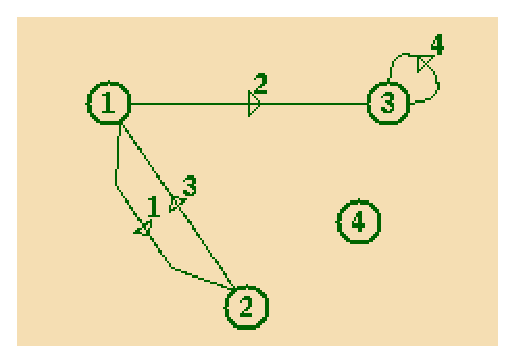
\psfig{file=foo.eps}}
  \caption{Small directed graph}
  \label{fig-foo}
\end{figure}

\subsubsection{Adjacency lists}\label{adjacency}

Another interesting representation often used by algorithms is the so
called \emph{adjacency lists}. It uses three row vectors, \texttt{lp},
\texttt{ls} and \texttt{la}. If $n$ is the number of nodes and $m$ is the number
of arcs of the graph,

\texttt{lp} is the pointer  array  (size = $n+1$)

\texttt{ls} is the node array (size = $m$)

\texttt{la} is the arc array (size = $m$).

If the graph is undirected, each edge corresponds to two arcs.

With this type of representation, it is easy to know the successors of
a node. Node number \texttt{i} has \texttt{lp(i+1)-lp(i)} successors
nodes with numbers from
\texttt{ls(lp(i))},\ldots,\texttt{ls(lp(i+1)-1)},
the corresponding arcs are 
\texttt{la(lp(i))},\ldots,\texttt{la(lp(i+1)-1)}.

The adjacency lists representation of the graph of figure~\ref{fig-foo}
is given below:

\begin{center}
\setlength{\unitlength}{0.00083300in}%
%
\begingroup\makeatletter\ifx\SetFigFont\undefined%
\gdef\SetFigFont#1#2#3#4#5{%
  \reset@font\fontsize{#1}{#2pt}%
  \fontfamily{#3}\fontseries{#4}\fontshape{#5}%
  \selectfont}%
\fi\endgroup%
\begin{picture}(2712,2421)(1201,-2323)
\thicklines
\put(2551,-1411){\framebox(450,450){}}
\put(1651,-2311){\framebox(450,450){}}
\put(1651,-1411){\framebox(450,450){}}
\put(2101,-1411){\framebox(450,450){}}
\put(3001,-1411){\framebox(450,450){}}
\put(2101,-2311){\framebox(450,450){}}
\put(2551,-2311){\framebox(450,450){}}
\put(3001,-2311){\framebox(450,450){}}
\put(2101,-511){\framebox(450,450){}}
\put(1651,-511){\framebox(450,450){}}
\put(2551,-511){\framebox(450,450){}}
\put(3001,-511){\framebox(450,450){}}
\put(3451,-511){\framebox(450,450){}}
\put(1876,-511){\vector( 0,-1){450}}
\put(1876,-1411){\line( 0,-1){450}}
\put(2326,-1411){\line( 0,-1){450}}
\put(2776,-1411){\line( 0,-1){450}}
\put(3226,-1411){\line( 0,-1){450}}
\put(2326,-511){\line( 0,-1){300}}
\put(2326,-811){\line( 1, 0){450}}
\put(2776,-811){\vector( 0,-1){150}}
\put(2776,-511){\line( 0,-1){150}}
\put(2776,-661){\line( 1, 0){450}}
\put(3226,-661){\vector( 0,-1){300}}
\put(1801,-361){\makebox(0,0)[lb]{\smash{\SetFigFont{12}{14.4}{\rmdefault}{\mddefault}{\updefault}1}}}
\put(2251,-361){\makebox(0,0)[lb]{\smash{\SetFigFont{12}{14.4}{\rmdefault}{\mddefault}{\updefault}3}}}
\put(2701,-361){\makebox(0,0)[lb]{\smash{\SetFigFont{12}{14.4}{\rmdefault}{\mddefault}{\updefault}4}}}
\put(3151,-361){\makebox(0,0)[lb]{\smash{\SetFigFont{12}{14.4}{\rmdefault}{\mddefault}{\updefault}5}}}
\put(3601,-361){\makebox(0,0)[lb]{\smash{\SetFigFont{12}{14.4}{\rmdefault}{\mddefault}{\updefault}5}}}
\put(1801,-1261){\makebox(0,0)[lb]{\smash{\SetFigFont{12}{14.4}{\rmdefault}{\mddefault}{\updefault}2}}}
\put(2251,-2161){\makebox(0,0)[lb]{\smash{\SetFigFont{12}{14.4}{\rmdefault}{\mddefault}{\updefault}2}}}
\put(2251,-1261){\makebox(0,0)[lb]{\smash{\SetFigFont{12}{14.4}{\rmdefault}{\mddefault}{\updefault}3}}}
\put(2701,-1261){\makebox(0,0)[lb]{\smash{\SetFigFont{12}{14.4}{\rmdefault}{\mddefault}{\updefault}1}}}
\put(3151,-1261){\makebox(0,0)[lb]{\smash{\SetFigFont{12}{14.4}{\rmdefault}{\mddefault}{\updefault}3}}}
\put(1801,-2161){\makebox(0,0)[lb]{\smash{\SetFigFont{12}{14.4}{\rmdefault}{\mddefault}{\updefault}1}}}
\put(2701,-2161){\makebox(0,0)[lb]{\smash{\SetFigFont{12}{14.4}{\rmdefault}{\mddefault}{\updefault}3}}}
\put(3151,-2161){\makebox(0,0)[lb]{\smash{\SetFigFont{12}{14.4}{\rmdefault}{\mddefault}{\updefault}4}}}
\put(1801, 14){\makebox(0,0)[lb]{\smash{\SetFigFont{10}{12.0}{\rmdefault}{\mddefault}{\updefault}1}}}
\put(2251, 14){\makebox(0,0)[lb]{\smash{\SetFigFont{10}{12.0}{\rmdefault}{\mddefault}{\updefault}2}}}
\put(2701, 14){\makebox(0,0)[lb]{\smash{\SetFigFont{10}{12.0}{\rmdefault}{\mddefault}{\updefault}3}}}
\put(3151, 14){\makebox(0,0)[lb]{\smash{\SetFigFont{10}{12.0}{\rmdefault}{\mddefault}{\updefault}4}}}
\put(3601, 14){\makebox(0,0)[lb]{\smash{\SetFigFont{10}{12.0}{\rmdefault}{\mddefault}{\updefault}5}}}
\put(1201,-286){\makebox(0,0)[lb]{\smash{\SetFigFont{14}{16.8}{\rmdefault}{\mddefault}{\updefault}lp}}}
\put(1201,-1186){\makebox(0,0)[lb]{\smash{\SetFigFont{14}{16.8}{\rmdefault}{\mddefault}{\updefault}ls}}}
\put(1201,-2086){\makebox(0,0)[lb]{\smash{\SetFigFont{14}{16.8}{\rmdefault}{\mddefault}{\updefault}la}}}
\end{picture}

\end{center}

The function used to compute the adjacency list
representation of a graph is \func{adj\_lists}.

\subsubsection{Node-arc matrix}

For a directed graph,
$n$ is the number of nodes and $m$ is the number of arcs of the
graph, the node-arc matrix $A$ is a $n\times m$ matrix:

if $A(i,j)=+1$, then node $i$ is the tail of arc $j$

if $A(i,j)=-1$, then node $i$ is the head of arc $i$.

If the graph is undirected and $m$ is the number of edges, 
the node-arc matrix $A$ is also a $n\times m$ matrix and:

if $A(i,j)=1$, then node $i$ is an end of edge $j$.

With this type of representation, it is impossible to have loops.

This matrix is represented in Scilab as a sparse matrix.

For instance, the node-arc matrix corresponding to figure~\ref{fig-foo},
with loop arc number 4 deleted is :
\[\left(\begin{array}{cccc}
 1 &  1 & -1 \\
-1 &  0 &  1 \\
 0 & -1 &  0 \\
 0 &  0 &  0 \\
\end{array}\right)\]

If the same graph is undirected, the matrix is:
\[\left(\begin{array}{cccc}
 1 &  1 &  1 \\
 1 &  0 &  1 \\
 0 &  1 &  0 \\
 0 &  0 &  0 \\
\end{array}\right)\]

The functions used to compute the node-arc matrix
of a graph, and to come back to a graph from the node-arc matrix are
\func{graph\_2\_mat} and \func{mat\_2\_graph}.

\subsubsection{Chained lists}

Another representation used by some algorithms is given by the
\emph{chained lists}. This representation uses four vectors,
\texttt{fe}, \texttt{che}, \texttt{fn} and \texttt{chn} which are
described below.

\texttt{e1=fe(i))} is the number of the first edge starting from node 
\texttt{i}

\texttt{e2=che(e1)} is the number of the second edge starting from
node \texttt{i}

\texttt{e3=che(e2)} is the number of the third edge starting from
node \texttt{i} 

and so on until the value is 0

\texttt{fn(i)} is the number of the first node reached from node i

\texttt{chn(i)} is the number of the node reached by edge
\texttt{che(i)}.

All this can be more clearly seen on figure~\ref{fig-chain}.

\begin{figure}
  \centerline{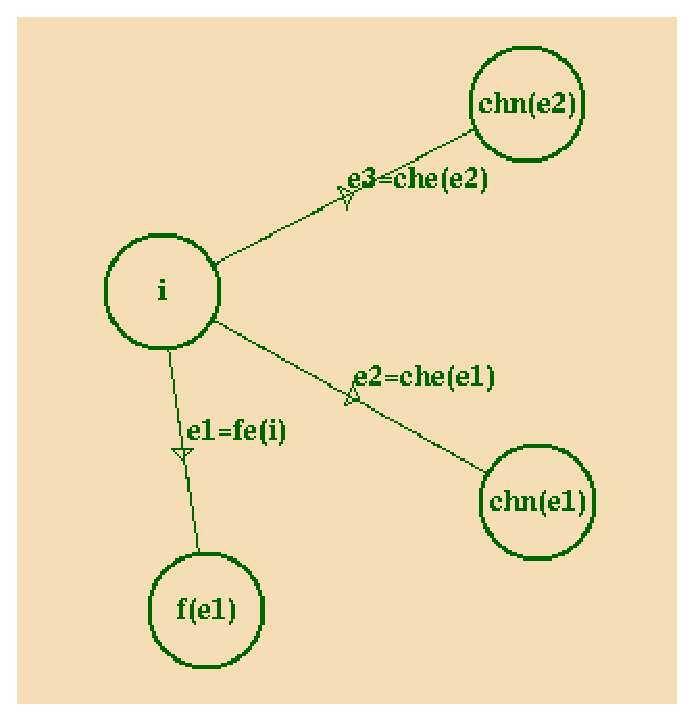
\psfig{file=chain.eps,width=5cm}}
  \caption{Chained list representation of graphs}
  \label{fig-chain}
\end{figure}

You can use the \func{chain\_struct} function to obtain the chained
lists representation of a graph from the adjacency lists representation
(see~\ref{adjacency}).

\section{Managing graphs}

We have seen (see~\ref{graph-list}) that a graph in Scilab is
represented by a graph list. This list contains everything needed to
define the graph, arcs, nodes, coordinates, colors, attributes, width of the
arcs, etc.

To create, load and save graphs in Scilab, you can only use Scilab
functions, handling graph lists, or you can use the Metanet window.
We describe here the first way. For the second way, see~\ref{xmetanet}.

\subsection{Creating graphs}\label{creating}

The standard function for making a graph list is
\func{make\_graph}.
The first argument is the name of the graph,
the second argument is a flag which can be 1 (directed graph) or 0
(undirected graph), the third argument is the number of nodes of the graph,
and the last two arguments are the tail
and head
vectors of 
the graph.

We have already seen that the graph named ``foo'' in figure~\ref{fig-foo}
can be created by the command:
\begin{verbatim}
g=make_graph('foo',1,4,[1 1 2 3],[2 3 1 3]);
\end{verbatim}

The simplest graph we can create in Metanet is:
\begin{verbatim}
g=make_graph('min',1,1,[1],[1]);
\end{verbatim}

It is directed, has one node and one loop arc on this node and can be
seen in figure~\ref{fig-min}.
\begin{figure}
  \centerline{
\psfig{file=min.eps}}
  \caption{Smallest directed graph}
  \label{fig-min}
\end{figure}

The following graph shown in figure~\ref{fig-ufoo} is the same as
the first graph we have created, but it 
is undirected:
\begin{verbatim}
g=make_graph('ufoo',0,4,[1 1 2 3],[2 3 1 3]);
\end{verbatim}

\begin{figure}
  \centerline{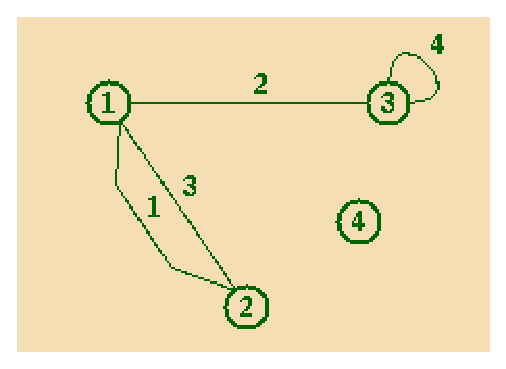
\psfig{file=ufoo.eps}}
  \caption{Small undirected graph}
  \label{fig-ufoo}
\end{figure}

You can also give 0 as the third argument of \func{make\_graph}
(number of nodes). This
means that \func{make\_graph} will compute itself from its last
arguments, the tail and head vectors, the number of nodes of the graph.
So, this graph has no isolated node and the nodes names are
taken from the numbers in tail and head vectors.
For instance, if you enter
\begin{verbatim}
g=make_graph('foo1',1,0,[1 1 4 3],[4 3 1 3]);
\end{verbatim}
the graph (shown in figure~\ref{fig-foo1}) has three nodes with names
1, 3 and 4, no isolated node and four edges. Note the difference with
the graph of figure~\ref{fig-foo}.

\begin{figure}
  \centerline{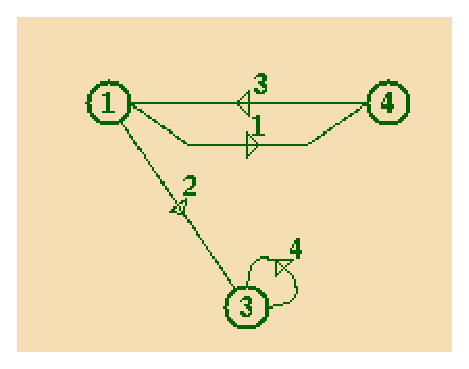
\psfig{file=foo1.eps}}
  \caption{Directed graph}
  \label{fig-foo1}
\end{figure}

The other elements of the graph list (see \ref{graph-list}) can be
entered by using the names of the elements. For instance, to give graph
``foo'' coordinates for the nodes, you can enter:
\begin{verbatim}
g=make_graph('foo',1,4,[1 1 2 3],[2 3 1 3]);
g('node_x')=[42 108 176 162];
g('node_y')=[36 134  36  93];
\end{verbatim}

Another simple example: if you want to transform the directed graph \texttt{g}
into
an undirected graph, you only have to do:
\begin{verbatim}
g('directed')=0;
\end{verbatim}

There is a wizard way to create a graph list ``by hands''
without using the 
\func{make\_graph} function. This can be useful when writing your
own Scilab functions.
You can use the Scilab function
\func{glist} which must have as many arguments as the elements of
the graph list (see~\ref{graph-list}).
This way can lead
to errors, because the list is somehow long. You can use the 
\func{check\_graph}
function to check if the graph list is correct.

\subsection{Loading and saving graphs}\label{loading}

Graphs are saved in ASCII files, called \emph{graph files}. The
structure of a graph file is given below:

{\small \begin{tabbing}
\texttt{GRAPH TYPE (0 = UNDIRECTED, 1 = DIRECTED), DEFAULTS (NODE
DIAMETER, NODE BORDER,}\\
\qquad first line continuing \texttt{ARC WIDTH, HILITED ARC WIDTH, FONTSIZE):}\\
$<$one line with above values$>$\\
\texttt{NUMBER OF ARCS:}\\
$<$one line with the number of arcs$>$\\
\texttt{NUMBER OF NODES:}\\
$<$one line with the number of nodes$>$\\
\texttt{****************************************}\\
\texttt{DESCRIPTION OF ARCS:}\\
\texttt{ARC NAME, TAIL NODE NAME, HEAD NODE NAME, COLOR, WIDTH, HIWIDTH, FONTSIZE}\\
\texttt{COST, MIN CAP, CAP, MAX CAP, LENGTH, Q WEIGHT, Q ORIGIN, WEIGHT}\\
$<$one blank line$>$\\
$<$two lines for each arc$>$\\
\texttt{****************************************}\\
\texttt{DESCRIPTION OF NODES:}\\
\texttt{NODE NAME, POSSIBLE TYPE (1 = SINK, 2 = SOURCE)}\\
\texttt{X, Y, COLOR, DIAMETER, BORDER, FONTSIZE}\\
\texttt{DEMAND}\\
$<$one blank line$>$\\
$<$three lines for each node$>$
\end{tabbing}}

For an undirected graph, \texttt{\small ARC} is replaced by
\texttt{\small EDGE}.  Moreover, the values of \texttt{\small NODE
DIAMETER}, \texttt{\small NODE BORDER}, \texttt{\small ARC WIDTH},
\texttt{\small HILITED ARC WIDTH} and \texttt{\small FONTSIZE} for the
graph, \texttt{\small COLOR}, \texttt{\small WIDTH}, \texttt{\small
HIWIDTH} and \texttt{\small FONTSIZE} for the arcs, and \texttt{\small
POSSIBLE TYPE}, \texttt{\small COLOR}, \texttt{\small DIAMETER},
\texttt{\small BORDER} and \texttt{\small FONTSIZE} for the nodes can
be omitted or equal to 0, then the default is used
(see~\ref{graph-list}).

A graph file has the extension ``graph''.

It is possible to create by hands a graph file and to load it into
Scilab, but it is a very cumbersome job. Programs are given to
generate graphs (see~\ref{generation}).

To load a graph into Scilab, use the \func{load\_graph} function.
Its argument is the absolute or relative pathname of the
graph file; if the ``graph'' extension is missing, it is
assumed. \func{load\_graph} returns the corresponding graph list.

For instance, to load the graph \texttt{foo}, which is in the current
directory, and put the corresponding graph list in the Scilab variable
\texttt{g}, do:

\texttt{g=load\_graph('foo');} or \texttt{g=load\_graph('foo.graph');}.

To load the graph \texttt{mesh100} given in the Scilab distribution,
do:

\texttt{g=load\_graph(SCI+'/demos/metanet/mesh100.graph');}

\medskip

To save a graph, use the \func{save\_graph} function. Its first
argument is the graph list, and its second argument is the name or the
pathname of the graph file; if the ``graph'' extension is missing, it is 
assumed. If the path  is the name of a directory, the name of the graph is
used as the name of the file.

For instance, the following command saves the graph \texttt{g} into
the graph file \texttt{foo.graph}:

\texttt{save\_graph(g,'foo.graph');}

\subsection{Plotting graphs}\label{plotting}

The fastest way to see a graph is to plot it in a Scilab graphical
window. We can use the \func{plot\_graph} function to do this.
Note that no interaction is possible with the displayed graph. If you
want to graphically modify the graph, use Metanet windows
(see~\ref{xmetanet}).

\section{Metanet windows}\label{xmetanet}

Metanet windows can be used to see the graphs and the
networks. It is a powerful tool to create and modify
graphs. You can have as many Metanet windows as you want
at the same time. Each Metanet window is an Unix process: the
communications between Scilab and the Metanet windows is made by using
the communication toolbox called GeCI. \textbf{Note} that at the
present time, Metanet windows only work on Unix operating system with
X Window.

By default, the size of Metanet windows is 1000 pixels by 1000
pixels. If you want to see big graphs, you have to change this values by
using X Window ressources. Put the new values in the ressources
\texttt{Metanet.drawWidth} and \texttt{Metanet.drawHeight} in a
standard ressource file (for instance \texttt{.Xdefaults} in your home
directory). For instance, if you want Metanet windows with a size of
2000 by 3000 pixels, puts the following lines in the ressource file:
\begin{verbatim}
Metanet.drawWidth: 2000
Metanet.drawHeight: 3000
\end{verbatim}

An important point is that there is no link between the graph
displayed in the Metanet window and the graphs loaded into Scilab. So,
when you have created or modified a graph in the Metanet window, you
have to save it as a graph file (see~\ref{loading}) and load it again
in Scilab. Conversely, when you have modified a graph in Scilab, you
have to display it again in the Metanet window by using the
\func{save\_graph} function (see~\ref{show}).

The philosophy is that computations are only made in Scilab and the
Metanet window is only used to display, create or modify graphs. So,
you can use Metanet toolbox without using Metanet windows.

Another way to see a graph is to plot it in a Scilab graphical window
(see~\ref{plotting}), but there is no possibility to modify the
displayed graph.

\subsection{Using the Metanet window}\label{window}

To open a Metanet window, use the \func{metanet} or
\func{show\_graph} Scilab functions (see~\ref{show}).

The Metanet window comes with three modes. When no graph is loaded,
you are in the \emph{Begin mode}. When a graph is loaded, you are in the
\emph{Study mode}. When you are creating a new graph or modifying a graph,
you are in the \emph{Modify mode}.

\subsubsection{Begin mode}

In this mode, you can load a graph or create a new one.

You will find below the description of the items of the menus.

\begin{description}
\item[Files]\ 
\begin{description}
  \item[New] Create a new graph. Prompt for the name of the graph and
	for its type (directed or not directed).
	Then you enter Modify Mode.
  \item[Load] Load a graph. Show the list of graphs in the default 
	directory. You have to choose one.
  \item[Directory] Change the default directory.
  \item[Quit] Quit Metanet.
\end{description}
\end{description}

\subsubsection{Study mode}

In this mode, you can load a graph, create a new one or work with an
already loaded graph.

With the left button of the mouse, you can highlight an arc or a node.

You will find below the description of the items of the menus.

\begin{description}
\item[Files]\ 
\begin{description}
  \item[New] Create a new graph. Prompt for the name of the graph and
	for its type  (directed or not directed).
	Then you enter Modify Mode.
  \item[Load] Load a graph. Show the list of graphs in the default
	directory. You  have to choose one.
  \item[Directory] Change the default directory.
  \item[Save As] Save the loaded graph with a new name in the default 
	directory.
  \item[Quit] Quit Metanet.
\end{description}
\item[Graph]\ 
\begin{description}
  \item[Characteristics] If there is an highlighted arc or node, print its
	characteristics, otherwise print the characteristics 
	of the graph.
  \item[Find Arc] Prompt for an arc name and highlight it. The viewport of the
	window is moved to display the arc if needed.
  \item[Find Node] Prompt for a node name and highlight it. The viewport of the
	window is moved to display the arc if needed.
  \item[Graphics] Change the scale. The default is 1.
  \item[Modify Graph] Enter Modify mode.
  \item[Use internal numbers as names] Use the consecutive internal numbers of
	arcs and nodes as names. This is useful 
	when working with Scilab.
  \item[Display arc names] Display arc names on the arcs.
  \item[Display node names] Display node names on the nodes.
\end{description}
\item[Redraw] Refresh the screen and redraw the graph.
\end{description}

\subsubsection{Modify mode}

In this mode, you can modify and save the graph.

\textbf{Note} that the only way to exit Modify Mode is to use the item 
\textbf{Quit Modify Mode} of \textbf{Modif} menu.


With the left button of the mouse, you can highlight an arc or a node.

With the right button of the mouse, you can modify the graph:
\begin{itemize}
\item if you click where there is no arc or node, a new node is created
\item if you click on a node and another node is highlighted, a new
	arc is created between the two nodes
\item if you click on a node and drag the mouse, the node is moved
\end{itemize}

You will find below the description of the items of the menus.

\begin{description}
\item[Files]\ 
\begin{description}
  \item[Directory] Change the default directory.
  \item[Save] Save the modified graph in the default directory. All 
	the arcs and nodes must have names.
  \item[Save As] Save the modified graph with a new name in the
	default directory.
	All the arcs and nodes must have names.
  \item[Quit] Do nothing.
\end{description}
\item[Graph]\ 
\begin{description}
  \item[Characteristics] If there is an highlighted arc or node, print its
	characteristics, otherwise print the characteristics 
	of the graph.
  \item[Find Arc] Prompt for an arc name and highlight it. The viewport of the
	window is moved to display the arc if needed.
  \item[Find Node]  Prompt for a node name and highlight it. The
	viewport of the window is moved to display the arc if needed.
  \item[Graphics] Change the scale. The default is 1.
  \item[Use internal numbers as names] Use the consecutive internal numbers of
	arcs and nodes as names. This is useful 
	when working with Scilab.
  \item[Display arc names] Display arc names on the arcs.
  \item[Display node names] Display node names on the nodes.
\end{description}
\item[Modify]\ 
\begin{description}
  \item[Attributes] Display the attributes of the highlighted arc or
	node. Then, they can be changed.
  \item[Delete] Delete the highlighted arc or node. 
	\textbf{Note:} there is no undelete.
  \item[Name] Name the highlighted arc or node.
  \item[Color] Give a color to the highlighted arc or node.
  \item[Create Loop] Create a loop arc on the highlighted node.
  \item[Create Sink] Transform the highlighted node into a sink.
  \item[Create Source] Transform the highlighted node into a source.
  \item[Remove Sink/Source] Transform the highlighted source or sink node
	into a plain node. It has no effect if the highlighted node is neither 
	a source nor a sink.
  \item[Automatic Name] Give the consecutive internal arc and node numbers as
	the names of arcs and nodes. This can be useful for a new graph.
	\textbf{Note} that if some arcs and nodes already have name, 
	they are replaced by the corresponding internal numbers.
  \item[Default Values] Change some default values:
	\begin{itemize}
                \item the default size of the font
                \item the default diameter of the nodes
                \item the default width of the border of the nodes
                \item the default width of the arcs
                \item the default width of the highlighted arcs
	\end{itemize}
  \item[Quit Modify Mode] Exit Modify Mode. If the graph has been
	modified, it must be saved first.
\end{description}
\item[Redraw] Refresh the screen and redraw the graph.
\end{description}

\subsection{Using the Metanet window from Scilab}\label{show}

The standard way of using the Metanet window is from
Scilab. Indeed, the Metanet window is opened only when needed as a
new process.

Many Metanet windows can be opened at the same time. Each Metanet
window has a number (integer starting from 1). One of these windows is
the \emph{current Metanet window}\index{current Metanet window}.

The \func{metanet} function opens a new Metanet window and returns its
number. A path can be given as an optional argument: it is the
directory where graph files are searched; by default, graph files are
searched in the working directory. The \func{metanet} function is
mainly used when we want to create a new graph.

We describe below the Scilab functions used in
conjunction with the Metanet window.

\subsubsection{Showing a graph}

The first thing we would like to do is to see the graph we are working
with: use the \func{show\_graph} function.

\texttt{show\_graph(g)} displays the graph \texttt{g} in the current
Metanet window. 
If there is no current Metanet window, a new Metanet window is created
and it becomes the current Metanet window.
If there is already a graph displayed in the current Metanet window,
the new graph is displayed instead. The number of the current Metanet
window, where the graph is displayed, is returned by \func{show\_graph}.

Two optional arguments can be given to \texttt{show\_graph(g)} after
the graph list.
If an optional argument is equal to the string 'new', a new 
Metanet window is created.
If an optional argument is a positive number, it is the value of the
scale factor when drawing the graph (see~\ref{window}).

For instance \texttt{show\_graph(g,'new',2)} displays the graph
\texttt{g} in a new Metanet window with the scale factor equal to 2.

\subsubsection{Showing arcs and nodes}

Another very useful thing to do is to distinguish a set of nodes
and/or a set of arcs in the displayed graph. This is done by
highlighting nodes and/or arc: use the \func{show\_arcs} and
\func{show\_nodes} functions.

The arguments of the \func{show\_arcs} and
\func{show\_nodes} functions are respectively a row vector of arc numbers (or
edge numbers if the graph is undirected) or a row vector of node
numbers. These sets of arcs and nodes are highlighted in the
current Metanet window. Note that the corresponding graph must be displayed in
this window, otherwise the numbers might not correspond to arcs or
nodes numbers (see~\ref{manage} for changing the current Metanet window).

By default, using one of these functions switch off any preceeding
highlighting. If you want to keep preceeding highlighting, use the
optional argument 'sup'.

For instance, the following commands displays the graph \texttt{g} and
highlights 3 arcs and 2 nodes:
\begin{verbatim}
show_graph(g)
show_arcs([1 10 3]); show_nodes([2 7],'sup')
\end{verbatim}

Note that another way to distinguish arcs and nodes in a displayed
graph is to give them colors. For that you have to use the elements 
\texttt{edge\_color} and \texttt{node\_color} of the graph list
(see~\ref{graph-list}). But you have to modify the graph list of the
graph and use \func{show\_graph} again to display the graph with
the new colors.

\subsubsection{Managing Metanet windows}\label{manage}

The \func{netwindow} function is used to change the current Metanet
window. For instance \texttt{netwindow(2)} chooses Metanet window
number 2 as the current Metanet window.

The \func{netwindows} function returns a list. Its first element is
the row vector of 
all the Metanet windows numbers and the second element is the number of the 
current Metanet window. This number is equal to 0 if no current Metanet
window exists.

In the following example, there are two Metanet windows with numbers 1
and 3 and the  Metanet window number 3 is the current Metanet window.
\begin{verbatim}
-->netwindows()
 ans  =
 
       ans(1)
 
!   1.    3. !
 
       ans(2)
 
    3.  
\end{verbatim}

\subsubsection{Synchronism}\label{synchro}

By default Metanet windows work with Scilab in asynchronous mode, 
\mbox{i.e.} Scilab
proceeds without waiting for graphics commands sent to Metanet windows to
terminate. This mode is the most efficient. But when running a lots of
graphics commands, problems can arise. For instance, you might
highlight a set of nodes in a bad Metanet window because the good one
has not yet appeared! So it is possible to use a synchronous
mode. Then Scilab waits until the functions dealing with the Metanet
windows have terminated. 

The \func{metanet\_sync} function is used to change the mode:
\texttt{metanet\_sync(0)} changes to asynchronous mode (default),
\texttt{metanet\_sync(1)} changes to synchronous mode, and
\texttt{metanet\_sync()} returns the current mode (0 = asynchronous,
1 = synchronous).

\section{Generating graphs and networks}\label{generation}

When working with graphs and particularly with networks, it is very
useful to generate them automatically.

The function \func{gen\_net} can be used in Metanet to generate
networks. It uses a triangulation method for generating a planar
connected graph and then uses the information of the user to give arcs
and nodes good values of costs and capacities.

\section{Computations on graphs and networks}

Most functions of the Metanet toolbox are used to make computations on
graphs and networks. We can distinguish four classes of such functions and
we will describe them briefly. For more information, see the on line
help.

\subsection{Graph manipulations and transformations}

You can use these functions to get information about graphs or to
modify existing graphs.

\begin{description}
\item[add\_edge] adds an edge or an arc between two nodes
\item[add\_node] adds a disconnected node to a graph
\item[arc\_graph] graph with nodes corresponding to arcs
\item[arc\_number] number of arcs of a graph
\item[contract\_edge] contracts edges between two nodes
\item[delete\_arcs] deletes all the arcs or edges between a set of nodes
\item[delete\_nodes] deletes nodes
\item[edge\_number] number of edges of a graph
\item[graph\_2\_mat] node-arc incidence matrix of a graph
\item[graph\_simp] converts a graph to a simple undirected graph
\item[graph\_sum] sum of two graphs
\item[graph\_union] union of two graphs
\item[line\_graph] graph with nodes corresponding to edges
\item[mat\_2\_graph] graph from node-arc incidence matrix
\item[node\_number] number of nodes of a graph
\item[nodes\_2\_path] path from a set of nodes
\item[path\_2\_nodes] set of nodes from a path
\item[split\_edge] splits an edge by inserting a node
\item[subgraph] subgraph of a graph 
\item[supernode] replaces a group of nodes with a single node
\end{description}

\subsection{Graph computations}

These functions are used to make standard computations on graphs.

\begin{description}
\item[articul] finds one or more articulation points 
\item[best\_match] best matching of a graph
\item[circuit] finds a circuit or the rank function in a directed graph
\item[con\_nodes] set of nodes of a connected component
\item[connex] connected components
\item[cycle\_basis] basis of cycle of a simple undirected graph
\item[find\_path] finds a path between two nodes
\item[girth] girth of a directed graph
\item[graph\_center] center of a graph
\item[graph\_complement] complement of a graph 
\item[graph\_diameter] diameter of a graph
\item[graph\_power] kth power of a directed 1-graph
\item[hamilton] hamiltonian circuit of a graph
\item[is\_connex] connectivity test
\item[max\_clique] maximum clique of a graph
\item[min\_weight\_tree] minimum weight spanning tree
\item[neighbors] nodes connected to a node
\item[nodes\_degrees] degrees of the nodes of a graph
\item[perfect\_match] min-cost perfect matching
\item[predecessors] tail nodes of incoming arcs of a node
\item[shortest\_path] shortest path
\item[strong\_con\_nodes] set of nodes of a strong connected component
\item[strong\_connex] strong connected components
\item[successors] head nodes of outgoing arcs of a node
\item[trans\_closure] transitive closure
\end{description}

\subsection{Network computations}

These functions make computations on networks. This means that the
graph has capacities and/or costs values on the edges.

\begin{description}
\item[max\_cap\_path] maximum capacity path
\item[max\_flow] maximum flow between two nodes
\item[min\_lcost\_cflow] minimum linear cost constrained flow
\item[min\_lcost\_flow1] minimum linear cost flow
\item[min\_lcost\_flow2] minimum linear cost flow
\item[min\_qcost\_flow] minimum quadratic cost flow
\end{description}

\subsection{Other computations}

These functions do not make computations directly on graphs and
networks, but there are strong links between them.

\begin{description}
\item[bandwr] bandwidth reduction for a sparse matrix
\item[convex\_hull] convex hull of a set of points in the plane
\item[knapsack] solves a 0-1 multiple knapsack problem
\item[mesh2d] triangulation of n points in the plane
\item[qassign] solves a quadratic assignment problem
\item[salesman] solves the travelling salesman problem
\end{description}

\newpage

\tableofcontents

\listoffigures

\documentclass[11pt]{article}

\textheight=23cm \textwidth=16cm
\topmargin=-1cm
\oddsidemargin=0pt \evensidemargin=0pt \marginparwidth=2cm

\usepackage{psfig}

\newcommand{\func}[1]{\texttt{#1}}

\title{Metanet User's Guide and Tutorial}
\author{Claude Gomez \and Maurice Goursat}
\date{Manual version 1.0 for Scilab 2.3}

\makeindex

\begin{document}

\maketitle

Metanet is a toolbox of Scilab for graphs and networks computations.
It comes as new
Scilab functions together with a graphical
window for displaying and modifying graphs.

You can use the Metanet toolbox in Scilab without using the graphical window
window at all,
\mbox{i.e.} without seeing the graphs or the networks you are working with.

\section{Representation of graphs}

The graphs handled by Metanet are directed or undirected multigraphs 
(loops are allowed).
A \emph{graph}\index{graph}
is a set of arcs and nodes. 

A graph must have at least one arc. 
We call \emph{arc}\index{arc} a directed link between two nodes. 
For instance the arc $(i,j)$ goes from \emph{tail}\index{tail}
node $i$ to \emph{head}\index{head}
node $j$. 
We call \emph{edge}\index{edge} the 
corresponding undirected link. A minimal way to represent a graph is to
give the number of nodes, the list of the tail nodes and the list of the
head nodes. Each node has a number and each arc has a number. The numbers
of nodes are consecutive and the number of arcs are consecutive. In Scilab,
these lists are represented by row vectors. So, if we call \texttt{tail} and
\texttt{head} these row vectors, the arc number $i$ goes from node
number \texttt{tail(i)} to node number \texttt{head(i)}. Moreover, 
the number of
nodes is necessary, because isolated nodes (without any arc) can exist. The
size of the vectors \texttt{tail} and \texttt{head} is the number of
edges of the graph. This is the standard representation of graphs in
Metanet as it is described in the graph list (see \ref{graph-list}).
There are functions to compute other representations better suited for
some algorithms (see \ref{representation}).

The distinction between edges\index{edge} and arcs is meaningful when
we 
deal with
undirected graphs. This distinction is not needed when we
only use the standard functions of Metanet. There is no distinction
between an \emph{arc}\index{arc} and a \emph{directed edge}\index{directed
edge}. 
We will often use indistinctly
these two terms.

A new object, the graph list data structure, is defined in
Scilab to handle graph. It is described below.

\subsection{The graph list data structure} \label{graph-list}

The graph list data structure is a typed list. 
As usual, the first element of this object is itself a list which
defines its 
type, \texttt{'graph'}, 
and all the access functions to the other elements.
The graph list has 33 elements (not counting the first one defining the type).
Only the first five elements must have a value in the list,
all the others can be given the empty vector \texttt{[]} as a value, and then a
default is used. These five required elements are:
\begin{description}
  \item[name] name of the graph (a string)
  \item[directed] flag equal to 1 if the graph is directed or equal
  to 0 if the graph is undirected
  \item[node\_number] number of nodes
  \item[tail] row vector of the tail node numbers
  \item[head] row vector of the head node numbers
\end{description}

A graph must at least have one arc, so \texttt{tail} and \texttt{head}
cannot be empty. 

See~\ref{representation} for the meaning of these elements.

For instance, you can define a graph list (see \ref{creating}) by
\begin{verbatim}
g=make_graph('min',1,1,[1],[1]);
\end{verbatim}
which is the simplest graph you can create (it is directed, has 
one node and one loop arc on this node).

With this type of description, we can have directed or undirected
multigraphs and multiple loops are allowed.

Each element of the list can be accessed by using its name.
For instance, if \texttt{g} is a graph list and
you want to get the \texttt{node\_number} element, you only have to type:

\texttt{g('node\_number')}

and if you want to change this value to 10, you only have to type:

\texttt{g('node\_number')=10}

The \func{check\_graph} function checks a graph list to see if
there are inconsistencies in its elements. Checking is not only
syntactic (number of elements of the list, compatible sizes 
of the vectors), but also semantic in the sense that 
\func{check\_graph} checks that \texttt{node\_number}, \texttt{tail} and 
\texttt{head} elements of the list can really represent a  graph.
This checking is automatically made when calling functions with a
graph list as an argument.

You will find below the description of all the elements of a graph list.

Each element is described by one or more lines.
The first lines gives the name of the element and
its definition, with its Scilab type if
needed.
The last line gives the default for elements that can have one.

The name of the element is used to access 
the elements
of the list.

\begin{description}
  \item[name] 

Name of the graph; a string with a maximum of 80
characters (\emph{REQUIRED}).

  \item[directed]

Flag giving the type of the graph; it is equal to 1 if the graph is
directed or equal to 0 is the graph is undirected (\emph{REQUIRED}).

  \item[node\_number]

Number of nodes (\emph{REQUIRED}).

  \item[tail]

Row vector of the tail node numbers (\emph{REQUIRED}).

  \item[head]

Row vector of the head node numbers (\emph{REQUIRED}).

  \item[node\_name]

Row vector of the node names; they must be different.

Default is the node numbers as node names.

  \item[node\_type]

Row vector of the node types; the type is an integer from 0 to 2:
\begin{itemize}
  \item[0:] plain node
  \item[1:] sink node
  \item[2:] source node
\end{itemize}

This element is mainly used to draw the nodes in the Metanet
window. A plain node is drawn as a circle. A sink or source node is a
node where extraneous flow goes out the node or goes into the node; it
is drawn differently (a circle with an outgoing or ingoing arrow).

Default is 0 (plain node).

  \item[node\_x]

Row vector of the x coordinates of the nodes.

Default is computed when showing the graph in the Metanet window
(see \ref{xmetanet}).

  \item[node\_y]

Row vector of the y coordinates of the nodes.

Default is computed when showing the graph in the Metanet window
(see \ref{xmetanet}).

  \item[node\_color]

Row vector of the node colors; 
the color is an integer from 0 to 16:
\begin{itemize}
  \item[0:] black
  \item[1:] navyblue
  \item[2:] blue
  \item[3:] skyblue
  \item[4:] aquamarine
  \item[5:] forestgreen
  \item[6:] green
  \item[7:] lightcyan
  \item[8:] cyan
  \item[9:] orange
  \item[10:] red
  \item[11:] magenta
  \item[12:] violet
  \item[13:] yellow
  \item[14:] gold
  \item[15:] beige
  \item[16:] white
\end{itemize}

Default is 0 (black).

  \item[node\_diam]

Row vector of the sizes of the node diameters in pixels (a node is
drawn as a circle).

Default is the value of element \texttt{default\_node\_diam}.

  \item[node\_border]

Row vector of the sizes of the node borders in pixels.

Default is the value of element \texttt{default\_node\_border}.

  \item[node\_font\_size]

Row vector of the sizes of the font used to draw the name or the label
of the node; 
you can choose
8, 10, 12, 14, 18 or 24.

Default is the value of element \texttt{default\_font\_size}.

  \item[node\_demand]

Row vector of the node demands.

The demands of the nodes are used in functions
\func{min\_lcost\_cflow}, 
\func{min\_lcost\_flow1}, \func{min\_lcost\_flow2},
\func{min\_qcost\_flow} and
\func{supernode}.

Default is 0.

  \item[edge\_name]

Row vector of the edge names; it is better that the names of the edges
are different, but this is not an error.

Default is the edge numbers as edge names.

  \item[edge\_color]

Row vector of the edge colors; 
the color is an integer from 0 to 16 (see \texttt{node\_color}).

Default is 0 (black).

  \item[edge\_width]

Row vector of the sizes of the edge widths in pixels.

Default is the value of element \texttt{default\_edge\_width}.

  \item[edge\_hi\_width]

Row vector of the sizes of the highlighted edge widths in pixels.

Default is the value of element \texttt{default\_edge\_hi\_width}.

  \item[edge\_font\_size]

Row vector of the sizes of the font used to draw the name or the label of
the edge; you 
can choose 8, 10, 12, 14, 18 or 24.

Default is the value of element \texttt{default\_font\_size}.

  \item[edge\_length]

Row vector of the edge lengths.

The lengths of the edges are used in functions \func{graph\_center}, 
\func{graph\_diameter},
\func{salesman} and \func{shortest\_path}.

Default is 0.

  \item[edge\_cost]

Row vector of the edge costs.

The costs of the edges are used in functions \func{min\_lcost\_cflow}, 
\func{min\_lcost\_flow1} and \func{min\_lcost\_flow2}.

Default is 0.

  \item[edge\_min\_cap]

Row vector of the edge minimum capacities.

The minimum capacities of the edges are used in functions \func{max\_flow}, 
\func{min\_lcost\_cflow}, 
\func{min\_lcost\_flow1}, \func{min\_lcost\_flow2} and
\func{min\_qcost\_flow}.

Default is 0.

  \item[edge\_max\_cap]

Row vector of the edge maximum capacities.

The maximum capacities of the edges are used in functions 
\func{max\_cap\_path}, 
\func{max\_flow}, 
\func{min\_lcost\_cflow}, 
\func{min\_lcost\_flow1}, \func{min\_lcost\_flow2} and
\func{min\_qcost\_flow}.

Default is 0.

  \item[edge\_q\_weight]

Row vector of the edge quadratic weights. It corresponds to $w(u)$ in
the value of the cost on edge $u$ with flow $\varphi(u)$:
$\frac{1}{2}w(u)(\varphi(u)-w_0(u))^2$.

The quadratic weights of the edges are used in function 
\func{min\_qcost\_flow}.

Default is 0.

  \item[edge\_q\_orig]

Row vector of the edge quadratic origins. It corresponds to $w_0(u)$ in
the value of the cost on edge $u$ with flow $\varphi(u)$:
$\frac{1}{2}w(u)(\varphi(u)-w_0(u))^2$.

The quadratic origins of the edges are used in function 
\func{min\_qcost\_flow}.

Default is 0.

  \item[edge\_weight]

Row vector of the edge weights.

The weights of the edges are used in function
\func{min\_weight\_tree}.

Default is 0.

  \item[default\_node\_diam]

Default size in pixels of the node diameters of the graph.

Default is 20.

  \item[default\_node\_border]

Default size in pixels of the node borders of the graph.

Default is 2.

  \item[default\_edge\_width]

Default size in pixels of the edge widths of the graph.

Default is 1.

  \item[default\_edge\_hi\_width]

Default size in pixels of the highlighted edge widths of the graph.

Default is 3.

  \item[default\_font\_size]

Default size of the font used to draw the names or the labels of nodes
and edges.

Default is 12.

  \item[node\_label]

Row vector of the node labels.

Node labels are used to draw a string in a node. It can be any string.
An empty label can be given as a blank string \texttt{' '}.

  \item[edge\_label]

Row vector of the edge labels.

Edge labels are used to draw a string on an edge. It can be any string.
An empty label can be given as a blank string \texttt{' '}.

\end{description}

\subsection{Various representations of graphs}\label{representation}

\subsubsection{Names and numbers}\label{number}

First of all, we need to distinguish between the name of a node or the
name of an
edge and their internal numbers. The name can be any string. Its is saved
in the graph file (see~\ref{loading}).
The internal
number is generated automatically when loading a graph. The nodes and
the edges have 
consecutive internal numbers starting from 1. 
When using the functions of Scilab working on graphs, all the
computations are made with internal numbers.

Often, the names are taken as the internal numbers. This is
the default when no names are given. In this case, the distinction
between a name and a number is not meaningful. Only the type of the
variable is not the same: the name is a string and the number is an integer.

In the following when
we talk about the number of a node or the number of an edge, we mean
the internal number.

\subsubsection{Tail head}

We have seen that the standard representation of a graph used by
Metanet is by the means of two row vectors
\texttt{tail} and
\texttt{head}:
arc number $i$ goes from node
number \texttt{tail(i)} to node number \texttt{head(i)}.
The size of these vectors is the same and is the number of arcs of the
graph.

Moreover the number of nodes must be given. It is greater than or
equal to the maximum integer number in \texttt{tail} and
\texttt{head}. If node numbers do not belong to \texttt{tail} and
\texttt{head} then there are isolated nodes.

If the graph is undirected, it is the same, but \texttt{tail(i)} and
\texttt{head(i)} can be exchanged.

This representation is very general and gives directed or undirected
multigraphs with possible loops and isolated nodes.

The standard function to create graphs is \func{make\_graph}
(see~ref{creating}). 
For instance, we can create a small directed graph with a loop and an
isolated (see figure~\ref{fig-foo}) node by using:
node number = 4,
tail = [1,1,2,3],
head = [2,3,1,3],\\
or in Scilab:
\texttt{g=make\_graph('foo',1,4,[1 1 2 3],[2 3 1 3]);}

\begin{figure}
  \centerline{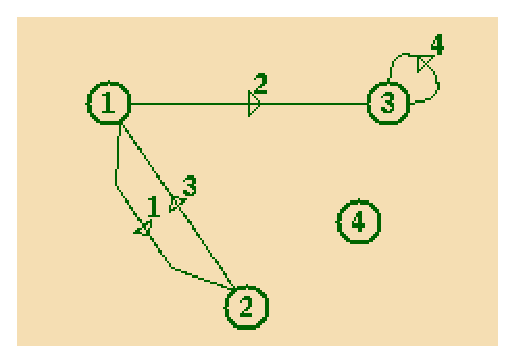
\psfig{file=foo.eps}}
  \caption{Small directed graph}
  \label{fig-foo}
\end{figure}

\subsubsection{Adjacency lists}\label{adjacency}

Another interesting representation often used by algorithms is the so
called \emph{adjacency lists}. It uses three row vectors, \texttt{lp},
\texttt{ls} and \texttt{la}. If $n$ is the number of nodes and $m$ is the number
of arcs of the graph,

\texttt{lp} is the pointer  array  (size = $n+1$)

\texttt{ls} is the node array (size = $m$)

\texttt{la} is the arc array (size = $m$).

If the graph is undirected, each edge corresponds to two arcs.

With this type of representation, it is easy to know the successors of
a node. Node number \texttt{i} has \texttt{lp(i+1)-lp(i)} successors
nodes with numbers from
\texttt{ls(lp(i))},\ldots,\texttt{ls(lp(i+1)-1)},
the corresponding arcs are 
\texttt{la(lp(i))},\ldots,\texttt{la(lp(i+1)-1)}.

The adjacency lists representation of the graph of figure~\ref{fig-foo}
is given below:

\begin{center}
\setlength{\unitlength}{0.00083300in}%
%
\begingroup\makeatletter\ifx\SetFigFont\undefined%
\gdef\SetFigFont#1#2#3#4#5{%
  \reset@font\fontsize{#1}{#2pt}%
  \fontfamily{#3}\fontseries{#4}\fontshape{#5}%
  \selectfont}%
\fi\endgroup%
\begin{picture}(2712,2421)(1201,-2323)
\thicklines
\put(2551,-1411){\framebox(450,450){}}
\put(1651,-2311){\framebox(450,450){}}
\put(1651,-1411){\framebox(450,450){}}
\put(2101,-1411){\framebox(450,450){}}
\put(3001,-1411){\framebox(450,450){}}
\put(2101,-2311){\framebox(450,450){}}
\put(2551,-2311){\framebox(450,450){}}
\put(3001,-2311){\framebox(450,450){}}
\put(2101,-511){\framebox(450,450){}}
\put(1651,-511){\framebox(450,450){}}
\put(2551,-511){\framebox(450,450){}}
\put(3001,-511){\framebox(450,450){}}
\put(3451,-511){\framebox(450,450){}}
\put(1876,-511){\vector( 0,-1){450}}
\put(1876,-1411){\line( 0,-1){450}}
\put(2326,-1411){\line( 0,-1){450}}
\put(2776,-1411){\line( 0,-1){450}}
\put(3226,-1411){\line( 0,-1){450}}
\put(2326,-511){\line( 0,-1){300}}
\put(2326,-811){\line( 1, 0){450}}
\put(2776,-811){\vector( 0,-1){150}}
\put(2776,-511){\line( 0,-1){150}}
\put(2776,-661){\line( 1, 0){450}}
\put(3226,-661){\vector( 0,-1){300}}
\put(1801,-361){\makebox(0,0)[lb]{\smash{\SetFigFont{12}{14.4}{\rmdefault}{\mddefault}{\updefault}1}}}
\put(2251,-361){\makebox(0,0)[lb]{\smash{\SetFigFont{12}{14.4}{\rmdefault}{\mddefault}{\updefault}3}}}
\put(2701,-361){\makebox(0,0)[lb]{\smash{\SetFigFont{12}{14.4}{\rmdefault}{\mddefault}{\updefault}4}}}
\put(3151,-361){\makebox(0,0)[lb]{\smash{\SetFigFont{12}{14.4}{\rmdefault}{\mddefault}{\updefault}5}}}
\put(3601,-361){\makebox(0,0)[lb]{\smash{\SetFigFont{12}{14.4}{\rmdefault}{\mddefault}{\updefault}5}}}
\put(1801,-1261){\makebox(0,0)[lb]{\smash{\SetFigFont{12}{14.4}{\rmdefault}{\mddefault}{\updefault}2}}}
\put(2251,-2161){\makebox(0,0)[lb]{\smash{\SetFigFont{12}{14.4}{\rmdefault}{\mddefault}{\updefault}2}}}
\put(2251,-1261){\makebox(0,0)[lb]{\smash{\SetFigFont{12}{14.4}{\rmdefault}{\mddefault}{\updefault}3}}}
\put(2701,-1261){\makebox(0,0)[lb]{\smash{\SetFigFont{12}{14.4}{\rmdefault}{\mddefault}{\updefault}1}}}
\put(3151,-1261){\makebox(0,0)[lb]{\smash{\SetFigFont{12}{14.4}{\rmdefault}{\mddefault}{\updefault}3}}}
\put(1801,-2161){\makebox(0,0)[lb]{\smash{\SetFigFont{12}{14.4}{\rmdefault}{\mddefault}{\updefault}1}}}
\put(2701,-2161){\makebox(0,0)[lb]{\smash{\SetFigFont{12}{14.4}{\rmdefault}{\mddefault}{\updefault}3}}}
\put(3151,-2161){\makebox(0,0)[lb]{\smash{\SetFigFont{12}{14.4}{\rmdefault}{\mddefault}{\updefault}4}}}
\put(1801, 14){\makebox(0,0)[lb]{\smash{\SetFigFont{10}{12.0}{\rmdefault}{\mddefault}{\updefault}1}}}
\put(2251, 14){\makebox(0,0)[lb]{\smash{\SetFigFont{10}{12.0}{\rmdefault}{\mddefault}{\updefault}2}}}
\put(2701, 14){\makebox(0,0)[lb]{\smash{\SetFigFont{10}{12.0}{\rmdefault}{\mddefault}{\updefault}3}}}
\put(3151, 14){\makebox(0,0)[lb]{\smash{\SetFigFont{10}{12.0}{\rmdefault}{\mddefault}{\updefault}4}}}
\put(3601, 14){\makebox(0,0)[lb]{\smash{\SetFigFont{10}{12.0}{\rmdefault}{\mddefault}{\updefault}5}}}
\put(1201,-286){\makebox(0,0)[lb]{\smash{\SetFigFont{14}{16.8}{\rmdefault}{\mddefault}{\updefault}lp}}}
\put(1201,-1186){\makebox(0,0)[lb]{\smash{\SetFigFont{14}{16.8}{\rmdefault}{\mddefault}{\updefault}ls}}}
\put(1201,-2086){\makebox(0,0)[lb]{\smash{\SetFigFont{14}{16.8}{\rmdefault}{\mddefault}{\updefault}la}}}
\end{picture}

\end{center}

The function used to compute the adjacency list
representation of a graph is \func{adj\_lists}.

\subsubsection{Node-arc matrix}

For a directed graph,
$n$ is the number of nodes and $m$ is the number of arcs of the
graph, the node-arc matrix $A$ is a $n\times m$ matrix:

if $A(i,j)=+1$, then node $i$ is the tail of arc $j$

if $A(i,j)=-1$, then node $i$ is the head of arc $i$.

If the graph is undirected and $m$ is the number of edges, 
the node-arc matrix $A$ is also a $n\times m$ matrix and:

if $A(i,j)=1$, then node $i$ is an end of edge $j$.

With this type of representation, it is impossible to have loops.

This matrix is represented in Scilab as a sparse matrix.

For instance, the node-arc matrix corresponding to figure~\ref{fig-foo},
with loop arc number 4 deleted is :
\[\left(\begin{array}{cccc}
 1 &  1 & -1 \\
-1 &  0 &  1 \\
 0 & -1 &  0 \\
 0 &  0 &  0 \\
\end{array}\right)\]

If the same graph is undirected, the matrix is:
\[\left(\begin{array}{cccc}
 1 &  1 &  1 \\
 1 &  0 &  1 \\
 0 &  1 &  0 \\
 0 &  0 &  0 \\
\end{array}\right)\]

The functions used to compute the node-arc matrix
of a graph, and to come back to a graph from the node-arc matrix are
\func{graph\_2\_mat} and \func{mat\_2\_graph}.

\subsubsection{Chained lists}

Another representation used by some algorithms is given by the
\emph{chained lists}. This representation uses four vectors,
\texttt{fe}, \texttt{che}, \texttt{fn} and \texttt{chn} which are
described below.

\texttt{e1=fe(i))} is the number of the first edge starting from node 
\texttt{i}

\texttt{e2=che(e1)} is the number of the second edge starting from
node \texttt{i}

\texttt{e3=che(e2)} is the number of the third edge starting from
node \texttt{i} 

and so on until the value is 0

\texttt{fn(i)} is the number of the first node reached from node i

\texttt{chn(i)} is the number of the node reached by edge
\texttt{che(i)}.

All this can be more clearly seen on figure~\ref{fig-chain}.

\begin{figure}
  \centerline{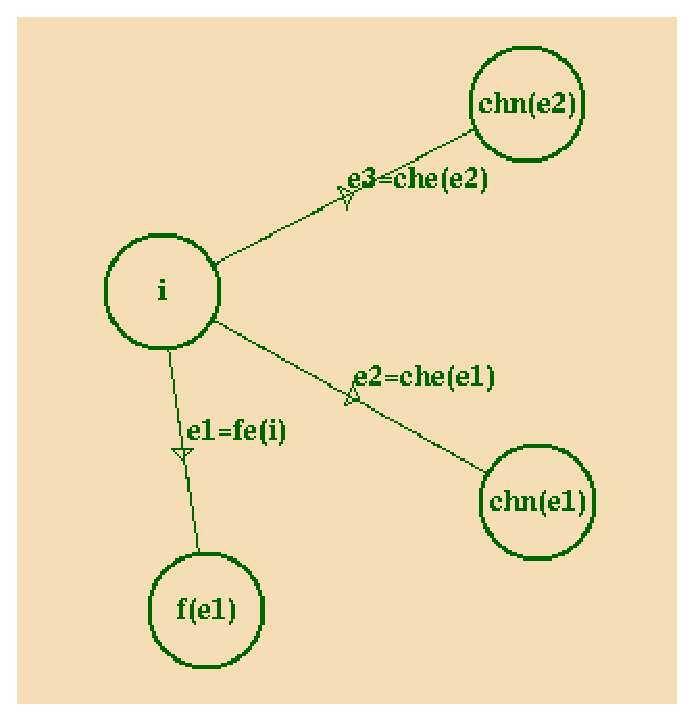
\psfig{file=chain.eps,width=5cm}}
  \caption{Chained list representation of graphs}
  \label{fig-chain}
\end{figure}

You can use the \func{chain\_struct} function to obtain the chained
lists representation of a graph from the adjacency lists representation
(see~\ref{adjacency}).

\section{Managing graphs}

We have seen (see~\ref{graph-list}) that a graph in Scilab is
represented by a graph list. This list contains everything needed to
define the graph, arcs, nodes, coordinates, colors, attributes, width of the
arcs, etc.

To create, load and save graphs in Scilab, you can only use Scilab
functions, handling graph lists, or you can use the Metanet window.
We describe here the first way. For the second way, see~\ref{xmetanet}.

\subsection{Creating graphs}\label{creating}

The standard function for making a graph list is
\func{make\_graph}.
The first argument is the name of the graph,
the second argument is a flag which can be 1 (directed graph) or 0
(undirected graph), the third argument is the number of nodes of the graph,
and the last two arguments are the tail
and head
vectors of 
the graph.

We have already seen that the graph named ``foo'' in figure~\ref{fig-foo}
can be created by the command:
\begin{verbatim}
g=make_graph('foo',1,4,[1 1 2 3],[2 3 1 3]);
\end{verbatim}

The simplest graph we can create in Metanet is:
\begin{verbatim}
g=make_graph('min',1,1,[1],[1]);
\end{verbatim}

It is directed, has one node and one loop arc on this node and can be
seen in figure~\ref{fig-min}.
\begin{figure}
  \centerline{
\psfig{file=min.eps}}
  \caption{Smallest directed graph}
  \label{fig-min}
\end{figure}

The following graph shown in figure~\ref{fig-ufoo} is the same as
the first graph we have created, but it 
is undirected:
\begin{verbatim}
g=make_graph('ufoo',0,4,[1 1 2 3],[2 3 1 3]);
\end{verbatim}

\begin{figure}
  \centerline{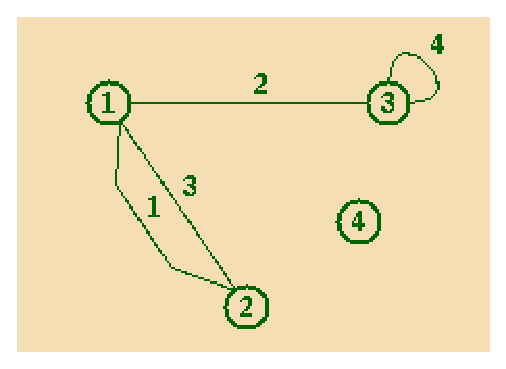
\psfig{file=ufoo.eps}}
  \caption{Small undirected graph}
  \label{fig-ufoo}
\end{figure}

You can also give 0 as the third argument of \func{make\_graph}
(number of nodes). This
means that \func{make\_graph} will compute itself from its last
arguments, the tail and head vectors, the number of nodes of the graph.
So, this graph has no isolated node and the nodes names are
taken from the numbers in tail and head vectors.
For instance, if you enter
\begin{verbatim}
g=make_graph('foo1',1,0,[1 1 4 3],[4 3 1 3]);
\end{verbatim}
the graph (shown in figure~\ref{fig-foo1}) has three nodes with names
1, 3 and 4, no isolated node and four edges. Note the difference with
the graph of figure~\ref{fig-foo}.

\begin{figure}
  \centerline{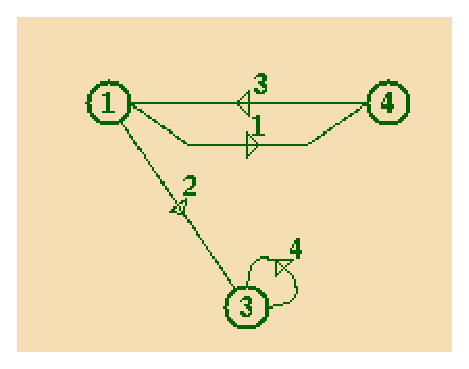
\psfig{file=foo1.eps}}
  \caption{Directed graph}
  \label{fig-foo1}
\end{figure}

The other elements of the graph list (see \ref{graph-list}) can be
entered by using the names of the elements. For instance, to give graph
``foo'' coordinates for the nodes, you can enter:
\begin{verbatim}
g=make_graph('foo',1,4,[1 1 2 3],[2 3 1 3]);
g('node_x')=[42 108 176 162];
g('node_y')=[36 134  36  93];
\end{verbatim}

Another simple example: if you want to transform the directed graph \texttt{g}
into
an undirected graph, you only have to do:
\begin{verbatim}
g('directed')=0;
\end{verbatim}

There is a wizard way to create a graph list ``by hands''
without using the 
\func{make\_graph} function. This can be useful when writing your
own Scilab functions.
You can use the Scilab function
\func{glist} which must have as many arguments as the elements of
the graph list (see~\ref{graph-list}).
This way can lead
to errors, because the list is somehow long. You can use the 
\func{check\_graph}
function to check if the graph list is correct.

\subsection{Loading and saving graphs}\label{loading}

Graphs are saved in ASCII files, called \emph{graph files}. The
structure of a graph file is given below:

{\small \begin{tabbing}
\texttt{GRAPH TYPE (0 = UNDIRECTED, 1 = DIRECTED), DEFAULTS (NODE
DIAMETER, NODE BORDER,}\\
\qquad first line continuing \texttt{ARC WIDTH, HILITED ARC WIDTH, FONTSIZE):}\\
$<$one line with above values$>$\\
\texttt{NUMBER OF ARCS:}\\
$<$one line with the number of arcs$>$\\
\texttt{NUMBER OF NODES:}\\
$<$one line with the number of nodes$>$\\
\texttt{****************************************}\\
\texttt{DESCRIPTION OF ARCS:}\\
\texttt{ARC NAME, TAIL NODE NAME, HEAD NODE NAME, COLOR, WIDTH, HIWIDTH, FONTSIZE}\\
\texttt{COST, MIN CAP, CAP, MAX CAP, LENGTH, Q WEIGHT, Q ORIGIN, WEIGHT}\\
$<$one blank line$>$\\
$<$two lines for each arc$>$\\
\texttt{****************************************}\\
\texttt{DESCRIPTION OF NODES:}\\
\texttt{NODE NAME, POSSIBLE TYPE (1 = SINK, 2 = SOURCE)}\\
\texttt{X, Y, COLOR, DIAMETER, BORDER, FONTSIZE}\\
\texttt{DEMAND}\\
$<$one blank line$>$\\
$<$three lines for each node$>$
\end{tabbing}}

For an undirected graph, \texttt{\small ARC} is replaced by
\texttt{\small EDGE}.  Moreover, the values of \texttt{\small NODE
DIAMETER}, \texttt{\small NODE BORDER}, \texttt{\small ARC WIDTH},
\texttt{\small HILITED ARC WIDTH} and \texttt{\small FONTSIZE} for the
graph, \texttt{\small COLOR}, \texttt{\small WIDTH}, \texttt{\small
HIWIDTH} and \texttt{\small FONTSIZE} for the arcs, and \texttt{\small
POSSIBLE TYPE}, \texttt{\small COLOR}, \texttt{\small DIAMETER},
\texttt{\small BORDER} and \texttt{\small FONTSIZE} for the nodes can
be omitted or equal to 0, then the default is used
(see~\ref{graph-list}).

A graph file has the extension ``graph''.

It is possible to create by hands a graph file and to load it into
Scilab, but it is a very cumbersome job. Programs are given to
generate graphs (see~\ref{generation}).

To load a graph into Scilab, use the \func{load\_graph} function.
Its argument is the absolute or relative pathname of the
graph file; if the ``graph'' extension is missing, it is
assumed. \func{load\_graph} returns the corresponding graph list.

For instance, to load the graph \texttt{foo}, which is in the current
directory, and put the corresponding graph list in the Scilab variable
\texttt{g}, do:

\texttt{g=load\_graph('foo');} or \texttt{g=load\_graph('foo.graph');}.

To load the graph \texttt{mesh100} given in the Scilab distribution,
do:

\texttt{g=load\_graph(SCI+'/demos/metanet/mesh100.graph');}

\medskip

To save a graph, use the \func{save\_graph} function. Its first
argument is the graph list, and its second argument is the name or the
pathname of the graph file; if the ``graph'' extension is missing, it is 
assumed. If the path  is the name of a directory, the name of the graph is
used as the name of the file.

For instance, the following command saves the graph \texttt{g} into
the graph file \texttt{foo.graph}:

\texttt{save\_graph(g,'foo.graph');}

\subsection{Plotting graphs}\label{plotting}

The fastest way to see a graph is to plot it in a Scilab graphical
window. We can use the \func{plot\_graph} function to do this.
Note that no interaction is possible with the displayed graph. If you
want to graphically modify the graph, use Metanet windows
(see~\ref{xmetanet}).

\section{Metanet windows}\label{xmetanet}

Metanet windows can be used to see the graphs and the
networks. It is a powerful tool to create and modify
graphs. You can have as many Metanet windows as you want
at the same time. Each Metanet window is an Unix process: the
communications between Scilab and the Metanet windows is made by using
the communication toolbox called GeCI. \textbf{Note} that at the
present time, Metanet windows only work on Unix operating system with
X Window.

By default, the size of Metanet windows is 1000 pixels by 1000
pixels. If you want to see big graphs, you have to change this values by
using X Window ressources. Put the new values in the ressources
\texttt{Metanet.drawWidth} and \texttt{Metanet.drawHeight} in a
standard ressource file (for instance \texttt{.Xdefaults} in your home
directory). For instance, if you want Metanet windows with a size of
2000 by 3000 pixels, puts the following lines in the ressource file:
\begin{verbatim}
Metanet.drawWidth: 2000
Metanet.drawHeight: 3000
\end{verbatim}

An important point is that there is no link between the graph
displayed in the Metanet window and the graphs loaded into Scilab. So,
when you have created or modified a graph in the Metanet window, you
have to save it as a graph file (see~\ref{loading}) and load it again
in Scilab. Conversely, when you have modified a graph in Scilab, you
have to display it again in the Metanet window by using the
\func{save\_graph} function (see~\ref{show}).

The philosophy is that computations are only made in Scilab and the
Metanet window is only used to display, create or modify graphs. So,
you can use Metanet toolbox without using Metanet windows.

Another way to see a graph is to plot it in a Scilab graphical window
(see~\ref{plotting}), but there is no possibility to modify the
displayed graph.

\subsection{Using the Metanet window}\label{window}

To open a Metanet window, use the \func{metanet} or
\func{show\_graph} Scilab functions (see~\ref{show}).

The Metanet window comes with three modes. When no graph is loaded,
you are in the \emph{Begin mode}. When a graph is loaded, you are in the
\emph{Study mode}. When you are creating a new graph or modifying a graph,
you are in the \emph{Modify mode}.

\subsubsection{Begin mode}

In this mode, you can load a graph or create a new one.

You will find below the description of the items of the menus.

\begin{description}
\item[Files]\ 
\begin{description}
  \item[New] Create a new graph. Prompt for the name of the graph and
	for its type (directed or not directed).
	Then you enter Modify Mode.
  \item[Load] Load a graph. Show the list of graphs in the default 
	directory. You have to choose one.
  \item[Directory] Change the default directory.
  \item[Quit] Quit Metanet.
\end{description}
\end{description}

\subsubsection{Study mode}

In this mode, you can load a graph, create a new one or work with an
already loaded graph.

With the left button of the mouse, you can highlight an arc or a node.

You will find below the description of the items of the menus.

\begin{description}
\item[Files]\ 
\begin{description}
  \item[New] Create a new graph. Prompt for the name of the graph and
	for its type  (directed or not directed).
	Then you enter Modify Mode.
  \item[Load] Load a graph. Show the list of graphs in the default
	directory. You  have to choose one.
  \item[Directory] Change the default directory.
  \item[Save As] Save the loaded graph with a new name in the default 
	directory.
  \item[Quit] Quit Metanet.
\end{description}
\item[Graph]\ 
\begin{description}
  \item[Characteristics] If there is an highlighted arc or node, print its
	characteristics, otherwise print the characteristics 
	of the graph.
  \item[Find Arc] Prompt for an arc name and highlight it. The viewport of the
	window is moved to display the arc if needed.
  \item[Find Node] Prompt for a node name and highlight it. The viewport of the
	window is moved to display the arc if needed.
  \item[Graphics] Change the scale. The default is 1.
  \item[Modify Graph] Enter Modify mode.
  \item[Use internal numbers as names] Use the consecutive internal numbers of
	arcs and nodes as names. This is useful 
	when working with Scilab.
  \item[Display arc names] Display arc names on the arcs.
  \item[Display node names] Display node names on the nodes.
\end{description}
\item[Redraw] Refresh the screen and redraw the graph.
\end{description}

\subsubsection{Modify mode}

In this mode, you can modify and save the graph.

\textbf{Note} that the only way to exit Modify Mode is to use the item 
\textbf{Quit Modify Mode} of \textbf{Modif} menu.


With the left button of the mouse, you can highlight an arc or a node.

With the right button of the mouse, you can modify the graph:
\begin{itemize}
\item if you click where there is no arc or node, a new node is created
\item if you click on a node and another node is highlighted, a new
	arc is created between the two nodes
\item if you click on a node and drag the mouse, the node is moved
\end{itemize}

You will find below the description of the items of the menus.

\begin{description}
\item[Files]\ 
\begin{description}
  \item[Directory] Change the default directory.
  \item[Save] Save the modified graph in the default directory. All 
	the arcs and nodes must have names.
  \item[Save As] Save the modified graph with a new name in the
	default directory.
	All the arcs and nodes must have names.
  \item[Quit] Do nothing.
\end{description}
\item[Graph]\ 
\begin{description}
  \item[Characteristics] If there is an highlighted arc or node, print its
	characteristics, otherwise print the characteristics 
	of the graph.
  \item[Find Arc] Prompt for an arc name and highlight it. The viewport of the
	window is moved to display the arc if needed.
  \item[Find Node]  Prompt for a node name and highlight it. The
	viewport of the window is moved to display the arc if needed.
  \item[Graphics] Change the scale. The default is 1.
  \item[Use internal numbers as names] Use the consecutive internal numbers of
	arcs and nodes as names. This is useful 
	when working with Scilab.
  \item[Display arc names] Display arc names on the arcs.
  \item[Display node names] Display node names on the nodes.
\end{description}
\item[Modify]\ 
\begin{description}
  \item[Attributes] Display the attributes of the highlighted arc or
	node. Then, they can be changed.
  \item[Delete] Delete the highlighted arc or node. 
	\textbf{Note:} there is no undelete.
  \item[Name] Name the highlighted arc or node.
  \item[Color] Give a color to the highlighted arc or node.
  \item[Create Loop] Create a loop arc on the highlighted node.
  \item[Create Sink] Transform the highlighted node into a sink.
  \item[Create Source] Transform the highlighted node into a source.
  \item[Remove Sink/Source] Transform the highlighted source or sink node
	into a plain node. It has no effect if the highlighted node is neither 
	a source nor a sink.
  \item[Automatic Name] Give the consecutive internal arc and node numbers as
	the names of arcs and nodes. This can be useful for a new graph.
	\textbf{Note} that if some arcs and nodes already have name, 
	they are replaced by the corresponding internal numbers.
  \item[Default Values] Change some default values:
	\begin{itemize}
                \item the default size of the font
                \item the default diameter of the nodes
                \item the default width of the border of the nodes
                \item the default width of the arcs
                \item the default width of the highlighted arcs
	\end{itemize}
  \item[Quit Modify Mode] Exit Modify Mode. If the graph has been
	modified, it must be saved first.
\end{description}
\item[Redraw] Refresh the screen and redraw the graph.
\end{description}

\subsection{Using the Metanet window from Scilab}\label{show}

The standard way of using the Metanet window is from
Scilab. Indeed, the Metanet window is opened only when needed as a
new process.

Many Metanet windows can be opened at the same time. Each Metanet
window has a number (integer starting from 1). One of these windows is
the \emph{current Metanet window}\index{current Metanet window}.

The \func{metanet} function opens a new Metanet window and returns its
number. A path can be given as an optional argument: it is the
directory where graph files are searched; by default, graph files are
searched in the working directory. The \func{metanet} function is
mainly used when we want to create a new graph.

We describe below the Scilab functions used in
conjunction with the Metanet window.

\subsubsection{Showing a graph}

The first thing we would like to do is to see the graph we are working
with: use the \func{show\_graph} function.

\texttt{show\_graph(g)} displays the graph \texttt{g} in the current
Metanet window. 
If there is no current Metanet window, a new Metanet window is created
and it becomes the current Metanet window.
If there is already a graph displayed in the current Metanet window,
the new graph is displayed instead. The number of the current Metanet
window, where the graph is displayed, is returned by \func{show\_graph}.

Two optional arguments can be given to \texttt{show\_graph(g)} after
the graph list.
If an optional argument is equal to the string 'new', a new 
Metanet window is created.
If an optional argument is a positive number, it is the value of the
scale factor when drawing the graph (see~\ref{window}).

For instance \texttt{show\_graph(g,'new',2)} displays the graph
\texttt{g} in a new Metanet window with the scale factor equal to 2.

\subsubsection{Showing arcs and nodes}

Another very useful thing to do is to distinguish a set of nodes
and/or a set of arcs in the displayed graph. This is done by
highlighting nodes and/or arc: use the \func{show\_arcs} and
\func{show\_nodes} functions.

The arguments of the \func{show\_arcs} and
\func{show\_nodes} functions are respectively a row vector of arc numbers (or
edge numbers if the graph is undirected) or a row vector of node
numbers. These sets of arcs and nodes are highlighted in the
current Metanet window. Note that the corresponding graph must be displayed in
this window, otherwise the numbers might not correspond to arcs or
nodes numbers (see~\ref{manage} for changing the current Metanet window).

By default, using one of these functions switch off any preceeding
highlighting. If you want to keep preceeding highlighting, use the
optional argument 'sup'.

For instance, the following commands displays the graph \texttt{g} and
highlights 3 arcs and 2 nodes:
\begin{verbatim}
show_graph(g)
show_arcs([1 10 3]); show_nodes([2 7],'sup')
\end{verbatim}

Note that another way to distinguish arcs and nodes in a displayed
graph is to give them colors. For that you have to use the elements 
\texttt{edge\_color} and \texttt{node\_color} of the graph list
(see~\ref{graph-list}). But you have to modify the graph list of the
graph and use \func{show\_graph} again to display the graph with
the new colors.

\subsubsection{Managing Metanet windows}\label{manage}

The \func{netwindow} function is used to change the current Metanet
window. For instance \texttt{netwindow(2)} chooses Metanet window
number 2 as the current Metanet window.

The \func{netwindows} function returns a list. Its first element is
the row vector of 
all the Metanet windows numbers and the second element is the number of the 
current Metanet window. This number is equal to 0 if no current Metanet
window exists.

In the following example, there are two Metanet windows with numbers 1
and 3 and the  Metanet window number 3 is the current Metanet window.
\begin{verbatim}
-->netwindows()
 ans  =
 
       ans(1)
 
!   1.    3. !
 
       ans(2)
 
    3.  
\end{verbatim}

\subsubsection{Synchronism}\label{synchro}

By default Metanet windows work with Scilab in asynchronous mode, 
\mbox{i.e.} Scilab
proceeds without waiting for graphics commands sent to Metanet windows to
terminate. This mode is the most efficient. But when running a lots of
graphics commands, problems can arise. For instance, you might
highlight a set of nodes in a bad Metanet window because the good one
has not yet appeared! So it is possible to use a synchronous
mode. Then Scilab waits until the functions dealing with the Metanet
windows have terminated. 

The \func{metanet\_sync} function is used to change the mode:
\texttt{metanet\_sync(0)} changes to asynchronous mode (default),
\texttt{metanet\_sync(1)} changes to synchronous mode, and
\texttt{metanet\_sync()} returns the current mode (0 = asynchronous,
1 = synchronous).

\section{Generating graphs and networks}\label{generation}

When working with graphs and particularly with networks, it is very
useful to generate them automatically.

The function \func{gen\_net} can be used in Metanet to generate
networks. It uses a triangulation method for generating a planar
connected graph and then uses the information of the user to give arcs
and nodes good values of costs and capacities.

\section{Computations on graphs and networks}

Most functions of the Metanet toolbox are used to make computations on
graphs and networks. We can distinguish four classes of such functions and
we will describe them briefly. For more information, see the on line
help.

\subsection{Graph manipulations and transformations}

You can use these functions to get information about graphs or to
modify existing graphs.

\begin{description}
\item[add\_edge] adds an edge or an arc between two nodes
\item[add\_node] adds a disconnected node to a graph
\item[arc\_graph] graph with nodes corresponding to arcs
\item[arc\_number] number of arcs of a graph
\item[contract\_edge] contracts edges between two nodes
\item[delete\_arcs] deletes all the arcs or edges between a set of nodes
\item[delete\_nodes] deletes nodes
\item[edge\_number] number of edges of a graph
\item[graph\_2\_mat] node-arc incidence matrix of a graph
\item[graph\_simp] converts a graph to a simple undirected graph
\item[graph\_sum] sum of two graphs
\item[graph\_union] union of two graphs
\item[line\_graph] graph with nodes corresponding to edges
\item[mat\_2\_graph] graph from node-arc incidence matrix
\item[node\_number] number of nodes of a graph
\item[nodes\_2\_path] path from a set of nodes
\item[path\_2\_nodes] set of nodes from a path
\item[split\_edge] splits an edge by inserting a node
\item[subgraph] subgraph of a graph 
\item[supernode] replaces a group of nodes with a single node
\end{description}

\subsection{Graph computations}

These functions are used to make standard computations on graphs.

\begin{description}
\item[articul] finds one or more articulation points 
\item[best\_match] best matching of a graph
\item[circuit] finds a circuit or the rank function in a directed graph
\item[con\_nodes] set of nodes of a connected component
\item[connex] connected components
\item[cycle\_basis] basis of cycle of a simple undirected graph
\item[find\_path] finds a path between two nodes
\item[girth] girth of a directed graph
\item[graph\_center] center of a graph
\item[graph\_complement] complement of a graph 
\item[graph\_diameter] diameter of a graph
\item[graph\_power] kth power of a directed 1-graph
\item[hamilton] hamiltonian circuit of a graph
\item[is\_connex] connectivity test
\item[max\_clique] maximum clique of a graph
\item[min\_weight\_tree] minimum weight spanning tree
\item[neighbors] nodes connected to a node
\item[nodes\_degrees] degrees of the nodes of a graph
\item[perfect\_match] min-cost perfect matching
\item[predecessors] tail nodes of incoming arcs of a node
\item[shortest\_path] shortest path
\item[strong\_con\_nodes] set of nodes of a strong connected component
\item[strong\_connex] strong connected components
\item[successors] head nodes of outgoing arcs of a node
\item[trans\_closure] transitive closure
\end{description}

\subsection{Network computations}

These functions make computations on networks. This means that the
graph has capacities and/or costs values on the edges.

\begin{description}
\item[max\_cap\_path] maximum capacity path
\item[max\_flow] maximum flow between two nodes
\item[min\_lcost\_cflow] minimum linear cost constrained flow
\item[min\_lcost\_flow1] minimum linear cost flow
\item[min\_lcost\_flow2] minimum linear cost flow
\item[min\_qcost\_flow] minimum quadratic cost flow
\end{description}

\subsection{Other computations}

These functions do not make computations directly on graphs and
networks, but there are strong links between them.

\begin{description}
\item[bandwr] bandwidth reduction for a sparse matrix
\item[convex\_hull] convex hull of a set of points in the plane
\item[knapsack] solves a 0-1 multiple knapsack problem
\item[mesh2d] triangulation of n points in the plane
\item[qassign] solves a quadratic assignment problem
\item[salesman] solves the travelling salesman problem
\end{description}

\newpage

\tableofcontents

\listoffigures

\documentclass[11pt]{article}

\textheight=23cm \textwidth=16cm
\topmargin=-1cm
\oddsidemargin=0pt \evensidemargin=0pt \marginparwidth=2cm

\usepackage{psfig}

\newcommand{\func}[1]{\texttt{#1}}

\title{Metanet User's Guide and Tutorial}
\author{Claude Gomez \and Maurice Goursat}
\date{Manual version 1.0 for Scilab 2.3}

\makeindex

\begin{document}

\maketitle

Metanet is a toolbox of Scilab for graphs and networks computations.
It comes as new
Scilab functions together with a graphical
window for displaying and modifying graphs.

You can use the Metanet toolbox in Scilab without using the graphical window
window at all,
\mbox{i.e.} without seeing the graphs or the networks you are working with.

\section{Representation of graphs}

The graphs handled by Metanet are directed or undirected multigraphs 
(loops are allowed).
A \emph{graph}\index{graph}
is a set of arcs and nodes. 

A graph must have at least one arc. 
We call \emph{arc}\index{arc} a directed link between two nodes. 
For instance the arc $(i,j)$ goes from \emph{tail}\index{tail}
node $i$ to \emph{head}\index{head}
node $j$. 
We call \emph{edge}\index{edge} the 
corresponding undirected link. A minimal way to represent a graph is to
give the number of nodes, the list of the tail nodes and the list of the
head nodes. Each node has a number and each arc has a number. The numbers
of nodes are consecutive and the number of arcs are consecutive. In Scilab,
these lists are represented by row vectors. So, if we call \texttt{tail} and
\texttt{head} these row vectors, the arc number $i$ goes from node
number \texttt{tail(i)} to node number \texttt{head(i)}. Moreover, 
the number of
nodes is necessary, because isolated nodes (without any arc) can exist. The
size of the vectors \texttt{tail} and \texttt{head} is the number of
edges of the graph. This is the standard representation of graphs in
Metanet as it is described in the graph list (see \ref{graph-list}).
There are functions to compute other representations better suited for
some algorithms (see \ref{representation}).

The distinction between edges\index{edge} and arcs is meaningful when
we 
deal with
undirected graphs. This distinction is not needed when we
only use the standard functions of Metanet. There is no distinction
between an \emph{arc}\index{arc} and a \emph{directed edge}\index{directed
edge}. 
We will often use indistinctly
these two terms.

A new object, the graph list data structure, is defined in
Scilab to handle graph. It is described below.

\subsection{The graph list data structure} \label{graph-list}

The graph list data structure is a typed list. 
As usual, the first element of this object is itself a list which
defines its 
type, \texttt{'graph'}, 
and all the access functions to the other elements.
The graph list has 33 elements (not counting the first one defining the type).
Only the first five elements must have a value in the list,
all the others can be given the empty vector \texttt{[]} as a value, and then a
default is used. These five required elements are:
\begin{description}
  \item[name] name of the graph (a string)
  \item[directed] flag equal to 1 if the graph is directed or equal
  to 0 if the graph is undirected
  \item[node\_number] number of nodes
  \item[tail] row vector of the tail node numbers
  \item[head] row vector of the head node numbers
\end{description}

A graph must at least have one arc, so \texttt{tail} and \texttt{head}
cannot be empty. 

See~\ref{representation} for the meaning of these elements.

For instance, you can define a graph list (see \ref{creating}) by
\begin{verbatim}
g=make_graph('min',1,1,[1],[1]);
\end{verbatim}
which is the simplest graph you can create (it is directed, has 
one node and one loop arc on this node).

With this type of description, we can have directed or undirected
multigraphs and multiple loops are allowed.

Each element of the list can be accessed by using its name.
For instance, if \texttt{g} is a graph list and
you want to get the \texttt{node\_number} element, you only have to type:

\texttt{g('node\_number')}

and if you want to change this value to 10, you only have to type:

\texttt{g('node\_number')=10}

The \func{check\_graph} function checks a graph list to see if
there are inconsistencies in its elements. Checking is not only
syntactic (number of elements of the list, compatible sizes 
of the vectors), but also semantic in the sense that 
\func{check\_graph} checks that \texttt{node\_number}, \texttt{tail} and 
\texttt{head} elements of the list can really represent a  graph.
This checking is automatically made when calling functions with a
graph list as an argument.

You will find below the description of all the elements of a graph list.

Each element is described by one or more lines.
The first lines gives the name of the element and
its definition, with its Scilab type if
needed.
The last line gives the default for elements that can have one.

The name of the element is used to access 
the elements
of the list.

\begin{description}
  \item[name] 

Name of the graph; a string with a maximum of 80
characters (\emph{REQUIRED}).

  \item[directed]

Flag giving the type of the graph; it is equal to 1 if the graph is
directed or equal to 0 is the graph is undirected (\emph{REQUIRED}).

  \item[node\_number]

Number of nodes (\emph{REQUIRED}).

  \item[tail]

Row vector of the tail node numbers (\emph{REQUIRED}).

  \item[head]

Row vector of the head node numbers (\emph{REQUIRED}).

  \item[node\_name]

Row vector of the node names; they must be different.

Default is the node numbers as node names.

  \item[node\_type]

Row vector of the node types; the type is an integer from 0 to 2:
\begin{itemize}
  \item[0:] plain node
  \item[1:] sink node
  \item[2:] source node
\end{itemize}

This element is mainly used to draw the nodes in the Metanet
window. A plain node is drawn as a circle. A sink or source node is a
node where extraneous flow goes out the node or goes into the node; it
is drawn differently (a circle with an outgoing or ingoing arrow).

Default is 0 (plain node).

  \item[node\_x]

Row vector of the x coordinates of the nodes.

Default is computed when showing the graph in the Metanet window
(see \ref{xmetanet}).

  \item[node\_y]

Row vector of the y coordinates of the nodes.

Default is computed when showing the graph in the Metanet window
(see \ref{xmetanet}).

  \item[node\_color]

Row vector of the node colors; 
the color is an integer from 0 to 16:
\begin{itemize}
  \item[0:] black
  \item[1:] navyblue
  \item[2:] blue
  \item[3:] skyblue
  \item[4:] aquamarine
  \item[5:] forestgreen
  \item[6:] green
  \item[7:] lightcyan
  \item[8:] cyan
  \item[9:] orange
  \item[10:] red
  \item[11:] magenta
  \item[12:] violet
  \item[13:] yellow
  \item[14:] gold
  \item[15:] beige
  \item[16:] white
\end{itemize}

Default is 0 (black).

  \item[node\_diam]

Row vector of the sizes of the node diameters in pixels (a node is
drawn as a circle).

Default is the value of element \texttt{default\_node\_diam}.

  \item[node\_border]

Row vector of the sizes of the node borders in pixels.

Default is the value of element \texttt{default\_node\_border}.

  \item[node\_font\_size]

Row vector of the sizes of the font used to draw the name or the label
of the node; 
you can choose
8, 10, 12, 14, 18 or 24.

Default is the value of element \texttt{default\_font\_size}.

  \item[node\_demand]

Row vector of the node demands.

The demands of the nodes are used in functions
\func{min\_lcost\_cflow}, 
\func{min\_lcost\_flow1}, \func{min\_lcost\_flow2},
\func{min\_qcost\_flow} and
\func{supernode}.

Default is 0.

  \item[edge\_name]

Row vector of the edge names; it is better that the names of the edges
are different, but this is not an error.

Default is the edge numbers as edge names.

  \item[edge\_color]

Row vector of the edge colors; 
the color is an integer from 0 to 16 (see \texttt{node\_color}).

Default is 0 (black).

  \item[edge\_width]

Row vector of the sizes of the edge widths in pixels.

Default is the value of element \texttt{default\_edge\_width}.

  \item[edge\_hi\_width]

Row vector of the sizes of the highlighted edge widths in pixels.

Default is the value of element \texttt{default\_edge\_hi\_width}.

  \item[edge\_font\_size]

Row vector of the sizes of the font used to draw the name or the label of
the edge; you 
can choose 8, 10, 12, 14, 18 or 24.

Default is the value of element \texttt{default\_font\_size}.

  \item[edge\_length]

Row vector of the edge lengths.

The lengths of the edges are used in functions \func{graph\_center}, 
\func{graph\_diameter},
\func{salesman} and \func{shortest\_path}.

Default is 0.

  \item[edge\_cost]

Row vector of the edge costs.

The costs of the edges are used in functions \func{min\_lcost\_cflow}, 
\func{min\_lcost\_flow1} and \func{min\_lcost\_flow2}.

Default is 0.

  \item[edge\_min\_cap]

Row vector of the edge minimum capacities.

The minimum capacities of the edges are used in functions \func{max\_flow}, 
\func{min\_lcost\_cflow}, 
\func{min\_lcost\_flow1}, \func{min\_lcost\_flow2} and
\func{min\_qcost\_flow}.

Default is 0.

  \item[edge\_max\_cap]

Row vector of the edge maximum capacities.

The maximum capacities of the edges are used in functions 
\func{max\_cap\_path}, 
\func{max\_flow}, 
\func{min\_lcost\_cflow}, 
\func{min\_lcost\_flow1}, \func{min\_lcost\_flow2} and
\func{min\_qcost\_flow}.

Default is 0.

  \item[edge\_q\_weight]

Row vector of the edge quadratic weights. It corresponds to $w(u)$ in
the value of the cost on edge $u$ with flow $\varphi(u)$:
$\frac{1}{2}w(u)(\varphi(u)-w_0(u))^2$.

The quadratic weights of the edges are used in function 
\func{min\_qcost\_flow}.

Default is 0.

  \item[edge\_q\_orig]

Row vector of the edge quadratic origins. It corresponds to $w_0(u)$ in
the value of the cost on edge $u$ with flow $\varphi(u)$:
$\frac{1}{2}w(u)(\varphi(u)-w_0(u))^2$.

The quadratic origins of the edges are used in function 
\func{min\_qcost\_flow}.

Default is 0.

  \item[edge\_weight]

Row vector of the edge weights.

The weights of the edges are used in function
\func{min\_weight\_tree}.

Default is 0.

  \item[default\_node\_diam]

Default size in pixels of the node diameters of the graph.

Default is 20.

  \item[default\_node\_border]

Default size in pixels of the node borders of the graph.

Default is 2.

  \item[default\_edge\_width]

Default size in pixels of the edge widths of the graph.

Default is 1.

  \item[default\_edge\_hi\_width]

Default size in pixels of the highlighted edge widths of the graph.

Default is 3.

  \item[default\_font\_size]

Default size of the font used to draw the names or the labels of nodes
and edges.

Default is 12.

  \item[node\_label]

Row vector of the node labels.

Node labels are used to draw a string in a node. It can be any string.
An empty label can be given as a blank string \texttt{' '}.

  \item[edge\_label]

Row vector of the edge labels.

Edge labels are used to draw a string on an edge. It can be any string.
An empty label can be given as a blank string \texttt{' '}.

\end{description}

\subsection{Various representations of graphs}\label{representation}

\subsubsection{Names and numbers}\label{number}

First of all, we need to distinguish between the name of a node or the
name of an
edge and their internal numbers. The name can be any string. Its is saved
in the graph file (see~\ref{loading}).
The internal
number is generated automatically when loading a graph. The nodes and
the edges have 
consecutive internal numbers starting from 1. 
When using the functions of Scilab working on graphs, all the
computations are made with internal numbers.

Often, the names are taken as the internal numbers. This is
the default when no names are given. In this case, the distinction
between a name and a number is not meaningful. Only the type of the
variable is not the same: the name is a string and the number is an integer.

In the following when
we talk about the number of a node or the number of an edge, we mean
the internal number.

\subsubsection{Tail head}

We have seen that the standard representation of a graph used by
Metanet is by the means of two row vectors
\texttt{tail} and
\texttt{head}:
arc number $i$ goes from node
number \texttt{tail(i)} to node number \texttt{head(i)}.
The size of these vectors is the same and is the number of arcs of the
graph.

Moreover the number of nodes must be given. It is greater than or
equal to the maximum integer number in \texttt{tail} and
\texttt{head}. If node numbers do not belong to \texttt{tail} and
\texttt{head} then there are isolated nodes.

If the graph is undirected, it is the same, but \texttt{tail(i)} and
\texttt{head(i)} can be exchanged.

This representation is very general and gives directed or undirected
multigraphs with possible loops and isolated nodes.

The standard function to create graphs is \func{make\_graph}
(see~ref{creating}). 
For instance, we can create a small directed graph with a loop and an
isolated (see figure~\ref{fig-foo}) node by using:
node number = 4,
tail = [1,1,2,3],
head = [2,3,1,3],\\
or in Scilab:
\texttt{g=make\_graph('foo',1,4,[1 1 2 3],[2 3 1 3]);}

\begin{figure}
  \centerline{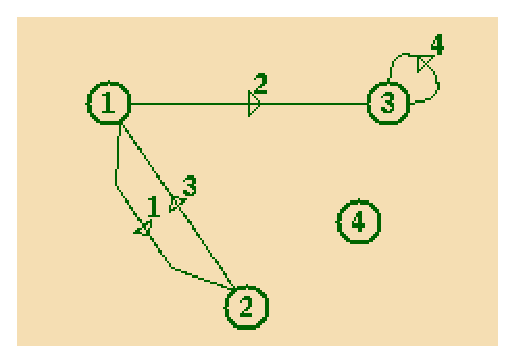
\psfig{file=foo.eps}}
  \caption{Small directed graph}
  \label{fig-foo}
\end{figure}

\subsubsection{Adjacency lists}\label{adjacency}

Another interesting representation often used by algorithms is the so
called \emph{adjacency lists}. It uses three row vectors, \texttt{lp},
\texttt{ls} and \texttt{la}. If $n$ is the number of nodes and $m$ is the number
of arcs of the graph,

\texttt{lp} is the pointer  array  (size = $n+1$)

\texttt{ls} is the node array (size = $m$)

\texttt{la} is the arc array (size = $m$).

If the graph is undirected, each edge corresponds to two arcs.

With this type of representation, it is easy to know the successors of
a node. Node number \texttt{i} has \texttt{lp(i+1)-lp(i)} successors
nodes with numbers from
\texttt{ls(lp(i))},\ldots,\texttt{ls(lp(i+1)-1)},
the corresponding arcs are 
\texttt{la(lp(i))},\ldots,\texttt{la(lp(i+1)-1)}.

The adjacency lists representation of the graph of figure~\ref{fig-foo}
is given below:

\begin{center}
\input{foo_adj.tex}
\end{center}

The function used to compute the adjacency list
representation of a graph is \func{adj\_lists}.

\subsubsection{Node-arc matrix}

For a directed graph,
$n$ is the number of nodes and $m$ is the number of arcs of the
graph, the node-arc matrix $A$ is a $n\times m$ matrix:

if $A(i,j)=+1$, then node $i$ is the tail of arc $j$

if $A(i,j)=-1$, then node $i$ is the head of arc $i$.

If the graph is undirected and $m$ is the number of edges, 
the node-arc matrix $A$ is also a $n\times m$ matrix and:

if $A(i,j)=1$, then node $i$ is an end of edge $j$.

With this type of representation, it is impossible to have loops.

This matrix is represented in Scilab as a sparse matrix.

For instance, the node-arc matrix corresponding to figure~\ref{fig-foo},
with loop arc number 4 deleted is :
\[\left(\begin{array}{cccc}
 1 &  1 & -1 \\
-1 &  0 &  1 \\
 0 & -1 &  0 \\
 0 &  0 &  0 \\
\end{array}\right)\]

If the same graph is undirected, the matrix is:
\[\left(\begin{array}{cccc}
 1 &  1 &  1 \\
 1 &  0 &  1 \\
 0 &  1 &  0 \\
 0 &  0 &  0 \\
\end{array}\right)\]

The functions used to compute the node-arc matrix
of a graph, and to come back to a graph from the node-arc matrix are
\func{graph\_2\_mat} and \func{mat\_2\_graph}.

\subsubsection{Chained lists}

Another representation used by some algorithms is given by the
\emph{chained lists}. This representation uses four vectors,
\texttt{fe}, \texttt{che}, \texttt{fn} and \texttt{chn} which are
described below.

\texttt{e1=fe(i))} is the number of the first edge starting from node 
\texttt{i}

\texttt{e2=che(e1)} is the number of the second edge starting from
node \texttt{i}

\texttt{e3=che(e2)} is the number of the third edge starting from
node \texttt{i} 

and so on until the value is 0

\texttt{fn(i)} is the number of the first node reached from node i

\texttt{chn(i)} is the number of the node reached by edge
\texttt{che(i)}.

All this can be more clearly seen on figure~\ref{fig-chain}.

\begin{figure}
  \centerline{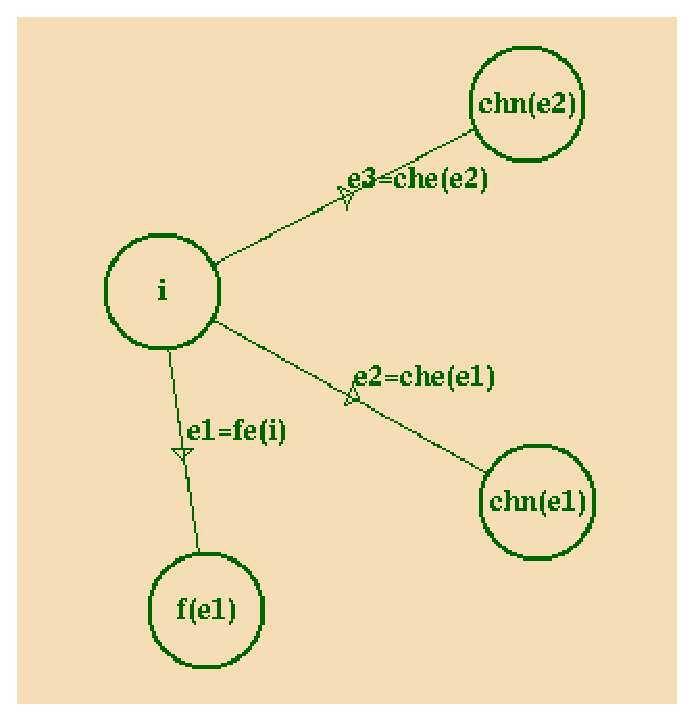
\psfig{file=chain.eps,width=5cm}}
  \caption{Chained list representation of graphs}
  \label{fig-chain}
\end{figure}

You can use the \func{chain\_struct} function to obtain the chained
lists representation of a graph from the adjacency lists representation
(see~\ref{adjacency}).

\section{Managing graphs}

We have seen (see~\ref{graph-list}) that a graph in Scilab is
represented by a graph list. This list contains everything needed to
define the graph, arcs, nodes, coordinates, colors, attributes, width of the
arcs, etc.

To create, load and save graphs in Scilab, you can only use Scilab
functions, handling graph lists, or you can use the Metanet window.
We describe here the first way. For the second way, see~\ref{xmetanet}.

\subsection{Creating graphs}\label{creating}

The standard function for making a graph list is
\func{make\_graph}.
The first argument is the name of the graph,
the second argument is a flag which can be 1 (directed graph) or 0
(undirected graph), the third argument is the number of nodes of the graph,
and the last two arguments are the tail
and head
vectors of 
the graph.

We have already seen that the graph named ``foo'' in figure~\ref{fig-foo}
can be created by the command:
\begin{verbatim}
g=make_graph('foo',1,4,[1 1 2 3],[2 3 1 3]);
\end{verbatim}

The simplest graph we can create in Metanet is:
\begin{verbatim}
g=make_graph('min',1,1,[1],[1]);
\end{verbatim}

It is directed, has one node and one loop arc on this node and can be
seen in figure~\ref{fig-min}.
\begin{figure}
  \centerline{
\psfig{file=min.eps}}
  \caption{Smallest directed graph}
  \label{fig-min}
\end{figure}

The following graph shown in figure~\ref{fig-ufoo} is the same as
the first graph we have created, but it 
is undirected:
\begin{verbatim}
g=make_graph('ufoo',0,4,[1 1 2 3],[2 3 1 3]);
\end{verbatim}

\begin{figure}
  \centerline{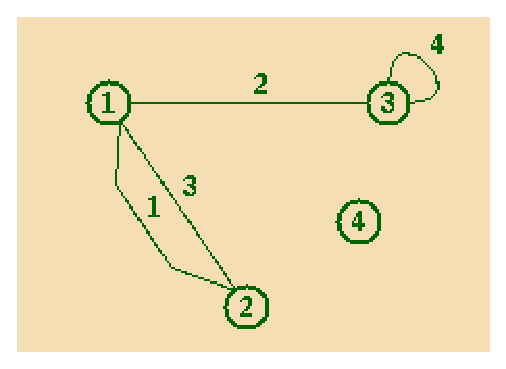
\psfig{file=ufoo.eps}}
  \caption{Small undirected graph}
  \label{fig-ufoo}
\end{figure}

You can also give 0 as the third argument of \func{make\_graph}
(number of nodes). This
means that \func{make\_graph} will compute itself from its last
arguments, the tail and head vectors, the number of nodes of the graph.
So, this graph has no isolated node and the nodes names are
taken from the numbers in tail and head vectors.
For instance, if you enter
\begin{verbatim}
g=make_graph('foo1',1,0,[1 1 4 3],[4 3 1 3]);
\end{verbatim}
the graph (shown in figure~\ref{fig-foo1}) has three nodes with names
1, 3 and 4, no isolated node and four edges. Note the difference with
the graph of figure~\ref{fig-foo}.

\begin{figure}
  \centerline{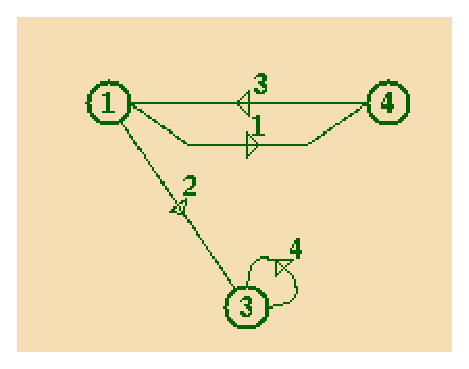
\psfig{file=foo1.eps}}
  \caption{Directed graph}
  \label{fig-foo1}
\end{figure}

The other elements of the graph list (see \ref{graph-list}) can be
entered by using the names of the elements. For instance, to give graph
``foo'' coordinates for the nodes, you can enter:
\begin{verbatim}
g=make_graph('foo',1,4,[1 1 2 3],[2 3 1 3]);
g('node_x')=[42 108 176 162];
g('node_y')=[36 134  36  93];
\end{verbatim}

Another simple example: if you want to transform the directed graph \texttt{g}
into
an undirected graph, you only have to do:
\begin{verbatim}
g('directed')=0;
\end{verbatim}

There is a wizard way to create a graph list ``by hands''
without using the 
\func{make\_graph} function. This can be useful when writing your
own Scilab functions.
You can use the Scilab function
\func{glist} which must have as many arguments as the elements of
the graph list (see~\ref{graph-list}).
This way can lead
to errors, because the list is somehow long. You can use the 
\func{check\_graph}
function to check if the graph list is correct.

\subsection{Loading and saving graphs}\label{loading}

Graphs are saved in ASCII files, called \emph{graph files}. The
structure of a graph file is given below:

{\small \begin{tabbing}
\texttt{GRAPH TYPE (0 = UNDIRECTED, 1 = DIRECTED), DEFAULTS (NODE
DIAMETER, NODE BORDER,}\\
\qquad first line continuing \texttt{ARC WIDTH, HILITED ARC WIDTH, FONTSIZE):}\\
$<$one line with above values$>$\\
\texttt{NUMBER OF ARCS:}\\
$<$one line with the number of arcs$>$\\
\texttt{NUMBER OF NODES:}\\
$<$one line with the number of nodes$>$\\
\texttt{****************************************}\\
\texttt{DESCRIPTION OF ARCS:}\\
\texttt{ARC NAME, TAIL NODE NAME, HEAD NODE NAME, COLOR, WIDTH, HIWIDTH, FONTSIZE}\\
\texttt{COST, MIN CAP, CAP, MAX CAP, LENGTH, Q WEIGHT, Q ORIGIN, WEIGHT}\\
$<$one blank line$>$\\
$<$two lines for each arc$>$\\
\texttt{****************************************}\\
\texttt{DESCRIPTION OF NODES:}\\
\texttt{NODE NAME, POSSIBLE TYPE (1 = SINK, 2 = SOURCE)}\\
\texttt{X, Y, COLOR, DIAMETER, BORDER, FONTSIZE}\\
\texttt{DEMAND}\\
$<$one blank line$>$\\
$<$three lines for each node$>$
\end{tabbing}}

For an undirected graph, \texttt{\small ARC} is replaced by
\texttt{\small EDGE}.  Moreover, the values of \texttt{\small NODE
DIAMETER}, \texttt{\small NODE BORDER}, \texttt{\small ARC WIDTH},
\texttt{\small HILITED ARC WIDTH} and \texttt{\small FONTSIZE} for the
graph, \texttt{\small COLOR}, \texttt{\small WIDTH}, \texttt{\small
HIWIDTH} and \texttt{\small FONTSIZE} for the arcs, and \texttt{\small
POSSIBLE TYPE}, \texttt{\small COLOR}, \texttt{\small DIAMETER},
\texttt{\small BORDER} and \texttt{\small FONTSIZE} for the nodes can
be omitted or equal to 0, then the default is used
(see~\ref{graph-list}).

A graph file has the extension ``graph''.

It is possible to create by hands a graph file and to load it into
Scilab, but it is a very cumbersome job. Programs are given to
generate graphs (see~\ref{generation}).

To load a graph into Scilab, use the \func{load\_graph} function.
Its argument is the absolute or relative pathname of the
graph file; if the ``graph'' extension is missing, it is
assumed. \func{load\_graph} returns the corresponding graph list.

For instance, to load the graph \texttt{foo}, which is in the current
directory, and put the corresponding graph list in the Scilab variable
\texttt{g}, do:

\texttt{g=load\_graph('foo');} or \texttt{g=load\_graph('foo.graph');}.

To load the graph \texttt{mesh100} given in the Scilab distribution,
do:

\texttt{g=load\_graph(SCI+'/demos/metanet/mesh100.graph');}

\medskip

To save a graph, use the \func{save\_graph} function. Its first
argument is the graph list, and its second argument is the name or the
pathname of the graph file; if the ``graph'' extension is missing, it is 
assumed. If the path  is the name of a directory, the name of the graph is
used as the name of the file.

For instance, the following command saves the graph \texttt{g} into
the graph file \texttt{foo.graph}:

\texttt{save\_graph(g,'foo.graph');}

\subsection{Plotting graphs}\label{plotting}

The fastest way to see a graph is to plot it in a Scilab graphical
window. We can use the \func{plot\_graph} function to do this.
Note that no interaction is possible with the displayed graph. If you
want to graphically modify the graph, use Metanet windows
(see~\ref{xmetanet}).

\section{Metanet windows}\label{xmetanet}

Metanet windows can be used to see the graphs and the
networks. It is a powerful tool to create and modify
graphs. You can have as many Metanet windows as you want
at the same time. Each Metanet window is an Unix process: the
communications between Scilab and the Metanet windows is made by using
the communication toolbox called GeCI. \textbf{Note} that at the
present time, Metanet windows only work on Unix operating system with
X Window.

By default, the size of Metanet windows is 1000 pixels by 1000
pixels. If you want to see big graphs, you have to change this values by
using X Window ressources. Put the new values in the ressources
\texttt{Metanet.drawWidth} and \texttt{Metanet.drawHeight} in a
standard ressource file (for instance \texttt{.Xdefaults} in your home
directory). For instance, if you want Metanet windows with a size of
2000 by 3000 pixels, puts the following lines in the ressource file:
\begin{verbatim}
Metanet.drawWidth: 2000
Metanet.drawHeight: 3000
\end{verbatim}

An important point is that there is no link between the graph
displayed in the Metanet window and the graphs loaded into Scilab. So,
when you have created or modified a graph in the Metanet window, you
have to save it as a graph file (see~\ref{loading}) and load it again
in Scilab. Conversely, when you have modified a graph in Scilab, you
have to display it again in the Metanet window by using the
\func{save\_graph} function (see~\ref{show}).

The philosophy is that computations are only made in Scilab and the
Metanet window is only used to display, create or modify graphs. So,
you can use Metanet toolbox without using Metanet windows.

Another way to see a graph is to plot it in a Scilab graphical window
(see~\ref{plotting}), but there is no possibility to modify the
displayed graph.

\subsection{Using the Metanet window}\label{window}

To open a Metanet window, use the \func{metanet} or
\func{show\_graph} Scilab functions (see~\ref{show}).

The Metanet window comes with three modes. When no graph is loaded,
you are in the \emph{Begin mode}. When a graph is loaded, you are in the
\emph{Study mode}. When you are creating a new graph or modifying a graph,
you are in the \emph{Modify mode}.

\subsubsection{Begin mode}

In this mode, you can load a graph or create a new one.

You will find below the description of the items of the menus.

\begin{description}
\item[Files]\ 
\begin{description}
  \item[New] Create a new graph. Prompt for the name of the graph and
	for its type (directed or not directed).
	Then you enter Modify Mode.
  \item[Load] Load a graph. Show the list of graphs in the default 
	directory. You have to choose one.
  \item[Directory] Change the default directory.
  \item[Quit] Quit Metanet.
\end{description}
\end{description}

\subsubsection{Study mode}

In this mode, you can load a graph, create a new one or work with an
already loaded graph.

With the left button of the mouse, you can highlight an arc or a node.

You will find below the description of the items of the menus.

\begin{description}
\item[Files]\ 
\begin{description}
  \item[New] Create a new graph. Prompt for the name of the graph and
	for its type  (directed or not directed).
	Then you enter Modify Mode.
  \item[Load] Load a graph. Show the list of graphs in the default
	directory. You  have to choose one.
  \item[Directory] Change the default directory.
  \item[Save As] Save the loaded graph with a new name in the default 
	directory.
  \item[Quit] Quit Metanet.
\end{description}
\item[Graph]\ 
\begin{description}
  \item[Characteristics] If there is an highlighted arc or node, print its
	characteristics, otherwise print the characteristics 
	of the graph.
  \item[Find Arc] Prompt for an arc name and highlight it. The viewport of the
	window is moved to display the arc if needed.
  \item[Find Node] Prompt for a node name and highlight it. The viewport of the
	window is moved to display the arc if needed.
  \item[Graphics] Change the scale. The default is 1.
  \item[Modify Graph] Enter Modify mode.
  \item[Use internal numbers as names] Use the consecutive internal numbers of
	arcs and nodes as names. This is useful 
	when working with Scilab.
  \item[Display arc names] Display arc names on the arcs.
  \item[Display node names] Display node names on the nodes.
\end{description}
\item[Redraw] Refresh the screen and redraw the graph.
\end{description}

\subsubsection{Modify mode}

In this mode, you can modify and save the graph.

\textbf{Note} that the only way to exit Modify Mode is to use the item 
\textbf{Quit Modify Mode} of \textbf{Modif} menu.


With the left button of the mouse, you can highlight an arc or a node.

With the right button of the mouse, you can modify the graph:
\begin{itemize}
\item if you click where there is no arc or node, a new node is created
\item if you click on a node and another node is highlighted, a new
	arc is created between the two nodes
\item if you click on a node and drag the mouse, the node is moved
\end{itemize}

You will find below the description of the items of the menus.

\begin{description}
\item[Files]\ 
\begin{description}
  \item[Directory] Change the default directory.
  \item[Save] Save the modified graph in the default directory. All 
	the arcs and nodes must have names.
  \item[Save As] Save the modified graph with a new name in the
	default directory.
	All the arcs and nodes must have names.
  \item[Quit] Do nothing.
\end{description}
\item[Graph]\ 
\begin{description}
  \item[Characteristics] If there is an highlighted arc or node, print its
	characteristics, otherwise print the characteristics 
	of the graph.
  \item[Find Arc] Prompt for an arc name and highlight it. The viewport of the
	window is moved to display the arc if needed.
  \item[Find Node]  Prompt for a node name and highlight it. The
	viewport of the window is moved to display the arc if needed.
  \item[Graphics] Change the scale. The default is 1.
  \item[Use internal numbers as names] Use the consecutive internal numbers of
	arcs and nodes as names. This is useful 
	when working with Scilab.
  \item[Display arc names] Display arc names on the arcs.
  \item[Display node names] Display node names on the nodes.
\end{description}
\item[Modify]\ 
\begin{description}
  \item[Attributes] Display the attributes of the highlighted arc or
	node. Then, they can be changed.
  \item[Delete] Delete the highlighted arc or node. 
	\textbf{Note:} there is no undelete.
  \item[Name] Name the highlighted arc or node.
  \item[Color] Give a color to the highlighted arc or node.
  \item[Create Loop] Create a loop arc on the highlighted node.
  \item[Create Sink] Transform the highlighted node into a sink.
  \item[Create Source] Transform the highlighted node into a source.
  \item[Remove Sink/Source] Transform the highlighted source or sink node
	into a plain node. It has no effect if the highlighted node is neither 
	a source nor a sink.
  \item[Automatic Name] Give the consecutive internal arc and node numbers as
	the names of arcs and nodes. This can be useful for a new graph.
	\textbf{Note} that if some arcs and nodes already have name, 
	they are replaced by the corresponding internal numbers.
  \item[Default Values] Change some default values:
	\begin{itemize}
                \item the default size of the font
                \item the default diameter of the nodes
                \item the default width of the border of the nodes
                \item the default width of the arcs
                \item the default width of the highlighted arcs
	\end{itemize}
  \item[Quit Modify Mode] Exit Modify Mode. If the graph has been
	modified, it must be saved first.
\end{description}
\item[Redraw] Refresh the screen and redraw the graph.
\end{description}

\subsection{Using the Metanet window from Scilab}\label{show}

The standard way of using the Metanet window is from
Scilab. Indeed, the Metanet window is opened only when needed as a
new process.

Many Metanet windows can be opened at the same time. Each Metanet
window has a number (integer starting from 1). One of these windows is
the \emph{current Metanet window}\index{current Metanet window}.

The \func{metanet} function opens a new Metanet window and returns its
number. A path can be given as an optional argument: it is the
directory where graph files are searched; by default, graph files are
searched in the working directory. The \func{metanet} function is
mainly used when we want to create a new graph.

We describe below the Scilab functions used in
conjunction with the Metanet window.

\subsubsection{Showing a graph}

The first thing we would like to do is to see the graph we are working
with: use the \func{show\_graph} function.

\texttt{show\_graph(g)} displays the graph \texttt{g} in the current
Metanet window. 
If there is no current Metanet window, a new Metanet window is created
and it becomes the current Metanet window.
If there is already a graph displayed in the current Metanet window,
the new graph is displayed instead. The number of the current Metanet
window, where the graph is displayed, is returned by \func{show\_graph}.

Two optional arguments can be given to \texttt{show\_graph(g)} after
the graph list.
If an optional argument is equal to the string 'new', a new 
Metanet window is created.
If an optional argument is a positive number, it is the value of the
scale factor when drawing the graph (see~\ref{window}).

For instance \texttt{show\_graph(g,'new',2)} displays the graph
\texttt{g} in a new Metanet window with the scale factor equal to 2.

\subsubsection{Showing arcs and nodes}

Another very useful thing to do is to distinguish a set of nodes
and/or a set of arcs in the displayed graph. This is done by
highlighting nodes and/or arc: use the \func{show\_arcs} and
\func{show\_nodes} functions.

The arguments of the \func{show\_arcs} and
\func{show\_nodes} functions are respectively a row vector of arc numbers (or
edge numbers if the graph is undirected) or a row vector of node
numbers. These sets of arcs and nodes are highlighted in the
current Metanet window. Note that the corresponding graph must be displayed in
this window, otherwise the numbers might not correspond to arcs or
nodes numbers (see~\ref{manage} for changing the current Metanet window).

By default, using one of these functions switch off any preceeding
highlighting. If you want to keep preceeding highlighting, use the
optional argument 'sup'.

For instance, the following commands displays the graph \texttt{g} and
highlights 3 arcs and 2 nodes:
\begin{verbatim}
show_graph(g)
show_arcs([1 10 3]); show_nodes([2 7],'sup')
\end{verbatim}

Note that another way to distinguish arcs and nodes in a displayed
graph is to give them colors. For that you have to use the elements 
\texttt{edge\_color} and \texttt{node\_color} of the graph list
(see~\ref{graph-list}). But you have to modify the graph list of the
graph and use \func{show\_graph} again to display the graph with
the new colors.

\subsubsection{Managing Metanet windows}\label{manage}

The \func{netwindow} function is used to change the current Metanet
window. For instance \texttt{netwindow(2)} chooses Metanet window
number 2 as the current Metanet window.

The \func{netwindows} function returns a list. Its first element is
the row vector of 
all the Metanet windows numbers and the second element is the number of the 
current Metanet window. This number is equal to 0 if no current Metanet
window exists.

In the following example, there are two Metanet windows with numbers 1
and 3 and the  Metanet window number 3 is the current Metanet window.
\begin{verbatim}
-->netwindows()
 ans  =
 
       ans(1)
 
!   1.    3. !
 
       ans(2)
 
    3.  
\end{verbatim}

\subsubsection{Synchronism}\label{synchro}

By default Metanet windows work with Scilab in asynchronous mode, 
\mbox{i.e.} Scilab
proceeds without waiting for graphics commands sent to Metanet windows to
terminate. This mode is the most efficient. But when running a lots of
graphics commands, problems can arise. For instance, you might
highlight a set of nodes in a bad Metanet window because the good one
has not yet appeared! So it is possible to use a synchronous
mode. Then Scilab waits until the functions dealing with the Metanet
windows have terminated. 

The \func{metanet\_sync} function is used to change the mode:
\texttt{metanet\_sync(0)} changes to asynchronous mode (default),
\texttt{metanet\_sync(1)} changes to synchronous mode, and
\texttt{metanet\_sync()} returns the current mode (0 = asynchronous,
1 = synchronous).

\section{Generating graphs and networks}\label{generation}

When working with graphs and particularly with networks, it is very
useful to generate them automatically.

The function \func{gen\_net} can be used in Metanet to generate
networks. It uses a triangulation method for generating a planar
connected graph and then uses the information of the user to give arcs
and nodes good values of costs and capacities.

\section{Computations on graphs and networks}

Most functions of the Metanet toolbox are used to make computations on
graphs and networks. We can distinguish four classes of such functions and
we will describe them briefly. For more information, see the on line
help.

\subsection{Graph manipulations and transformations}

You can use these functions to get information about graphs or to
modify existing graphs.

\begin{description}
\item[add\_edge] adds an edge or an arc between two nodes
\item[add\_node] adds a disconnected node to a graph
\item[arc\_graph] graph with nodes corresponding to arcs
\item[arc\_number] number of arcs of a graph
\item[contract\_edge] contracts edges between two nodes
\item[delete\_arcs] deletes all the arcs or edges between a set of nodes
\item[delete\_nodes] deletes nodes
\item[edge\_number] number of edges of a graph
\item[graph\_2\_mat] node-arc incidence matrix of a graph
\item[graph\_simp] converts a graph to a simple undirected graph
\item[graph\_sum] sum of two graphs
\item[graph\_union] union of two graphs
\item[line\_graph] graph with nodes corresponding to edges
\item[mat\_2\_graph] graph from node-arc incidence matrix
\item[node\_number] number of nodes of a graph
\item[nodes\_2\_path] path from a set of nodes
\item[path\_2\_nodes] set of nodes from a path
\item[split\_edge] splits an edge by inserting a node
\item[subgraph] subgraph of a graph 
\item[supernode] replaces a group of nodes with a single node
\end{description}

\subsection{Graph computations}

These functions are used to make standard computations on graphs.

\begin{description}
\item[articul] finds one or more articulation points 
\item[best\_match] best matching of a graph
\item[circuit] finds a circuit or the rank function in a directed graph
\item[con\_nodes] set of nodes of a connected component
\item[connex] connected components
\item[cycle\_basis] basis of cycle of a simple undirected graph
\item[find\_path] finds a path between two nodes
\item[girth] girth of a directed graph
\item[graph\_center] center of a graph
\item[graph\_complement] complement of a graph 
\item[graph\_diameter] diameter of a graph
\item[graph\_power] kth power of a directed 1-graph
\item[hamilton] hamiltonian circuit of a graph
\item[is\_connex] connectivity test
\item[max\_clique] maximum clique of a graph
\item[min\_weight\_tree] minimum weight spanning tree
\item[neighbors] nodes connected to a node
\item[nodes\_degrees] degrees of the nodes of a graph
\item[perfect\_match] min-cost perfect matching
\item[predecessors] tail nodes of incoming arcs of a node
\item[shortest\_path] shortest path
\item[strong\_con\_nodes] set of nodes of a strong connected component
\item[strong\_connex] strong connected components
\item[successors] head nodes of outgoing arcs of a node
\item[trans\_closure] transitive closure
\end{description}

\subsection{Network computations}

These functions make computations on networks. This means that the
graph has capacities and/or costs values on the edges.

\begin{description}
\item[max\_cap\_path] maximum capacity path
\item[max\_flow] maximum flow between two nodes
\item[min\_lcost\_cflow] minimum linear cost constrained flow
\item[min\_lcost\_flow1] minimum linear cost flow
\item[min\_lcost\_flow2] minimum linear cost flow
\item[min\_qcost\_flow] minimum quadratic cost flow
\end{description}

\subsection{Other computations}

These functions do not make computations directly on graphs and
networks, but there are strong links between them.

\begin{description}
\item[bandwr] bandwidth reduction for a sparse matrix
\item[convex\_hull] convex hull of a set of points in the plane
\item[knapsack] solves a 0-1 multiple knapsack problem
\item[mesh2d] triangulation of n points in the plane
\item[qassign] solves a quadratic assignment problem
\item[salesman] solves the travelling salesman problem
\end{description}

\newpage

\tableofcontents

\listoffigures

\input{metanet.ind}

\end{document}


\end{document}


\end{document}


\end{document}
